\documentclass[12pt]{article}
\usepackage{mathtools}
\usepackage{tabularx}
\usepackage[utf8]{inputenc}
\usepackage[T1]{fontenc}
\usepackage{natbib}
\usepackage{graphicx}
\usepackage[italian]{babel}
\usepackage{hyperref}
\usepackage{textcomp}
\usepackage{float}
\usepackage[dvipsnames]{xcolor}
\usepackage{sectsty}
\usepackage{pdfpages}
\usepackage{amssymb}
\usepackage{amsmath}
\usepackage{amsthm}
\usepackage{enumitem}
\usepackage{bm}
\usepackage{geometry}
\usepackage{bigints}
\usepackage{mdframed}
\paragraphfont{\color{red}}

\setcounter{tocdepth}{4}
\setcounter{secnumdepth}{4}
\graphicspath{{./Img/}}
\newgeometry{vmargin={15mm}, hmargin={12mm}}   % set the margins

\newcommand{\myparagraph}[1]{\paragraph{#1}\mbox{}\\}
\newcommand{\framedImg}[2]
{
	\begin{figure}[H]
		\centering
		\begin{tabular}{c}
			\framebox{\includegraphics[width=.#1\textwidth]{#2}}
		\end{tabular}
	\end{figure}
}

\newcommand{\nFramedImg}[2]
{
	\begin{figure}[H]
		\centering
		\begin{tabular}{c}
			\includegraphics[width=.#1\textwidth]{#2}
		\end{tabular}
	\end{figure}
}


\newcommand{\definizione}[2]{\textbf{\textit{\textcolor{OliveGreen}{def. #1}}}\label{#2}}

\newcommand{\importante}[1]{\textbf{\textit{\textcolor{Red}{#1}}}}

\title{
    \begin{figure}[ht!]
        \centering
        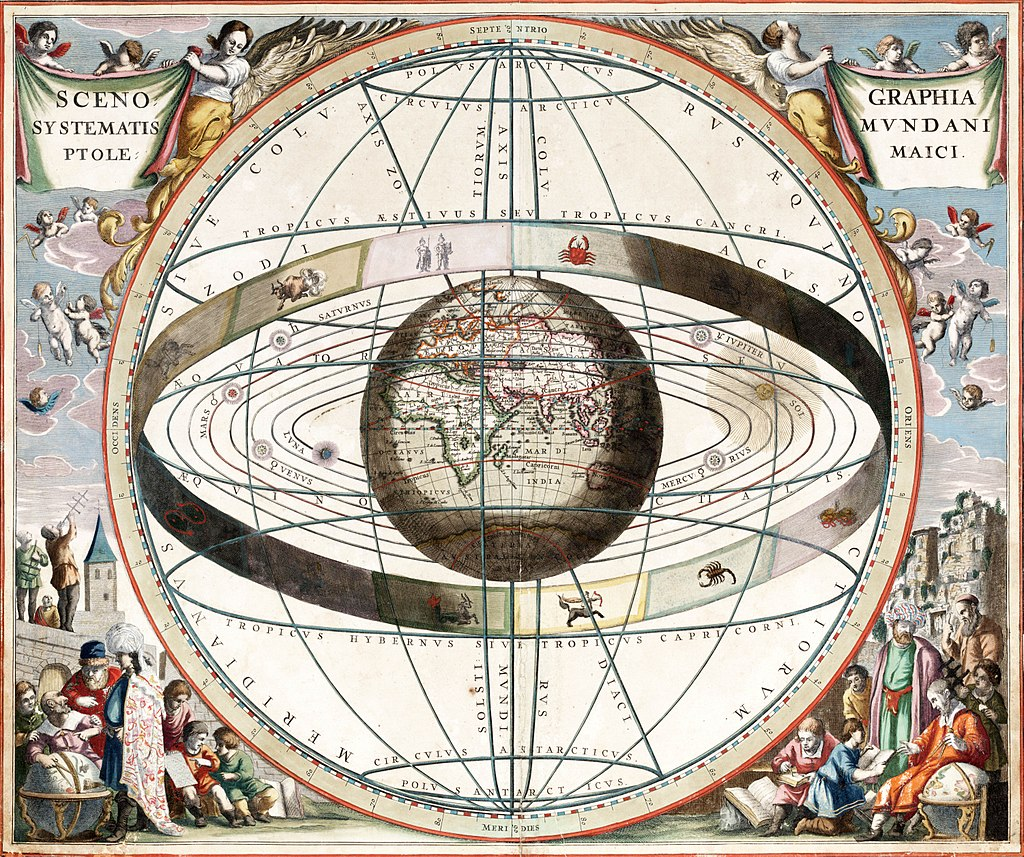
\includegraphics[width=.5\textwidth]{LOGO1}
    \end{figure}
    \bigskip
    Fisica
}
\author{UNITN - Lazzerini Thomas, Cappelletti Samuele}
\date{Marzo 2021}

\begin{document}
%    \sffamily
    \maketitle
    \vfill

    \begin{center}
        Nel presente documento sono presenti gli appunti relativi alla teoria del corso "\textbf{Fisica}" dell'anno \textbf{2021-2022} tenuto dal \textbf{professor Iuppa}).\\
    \end{center}

    \newpage

    \tableofcontents

    \newpage

	\section{Formulario}
	\subsection{Unità di misura}
		\begin{align*}
			& T && => && 10^{12}&&   && G && => && 10^{9}\\
			& M && => && 10^{6}&&   && k && => && 10^{3}\\
			& m && => && 10^{-3}&&   && \mu && => && 10^{-6}\\
			& n && => && 10^{-9}&&   && p && => && 10^{-12}\\
		\end{align*}
	
	\section{Introduzione}
	\subsection{Il metodo sperimentale}
		Distingue discipline sperimentali da discipline non sperimentali. Si compone di diverse fasi:
		\begin{enumerate}
			\item \textbf{formulazione ipotesi}: si fa un'\textbf{ipostesi descrittiva} (in \textbf{linguaggio matematico}) della porzione di mondo che si vuole analizzare, di conseguenza si decide di \textbf{non considerare} altre caratteristiche del mondo che non centrano con l'ipotesi che stiamo formulando;
			\item \textbf{esperimento}: si va a ricreare una situazione dove l'aspetto che vogliamo analizzare è \textbf{sicuramente presente} e \textbf{influenzato il meno possibile da fattori esterni};
			\item \textbf{esecuzione dell'esperimento}: si verifica l'ipotesi, formulata in modo matematico, confrontando i valori ottenuti con l'esperimento con quelli che si ottengono dalla nostra ipotesi.
			\medskip\\
		\end{enumerate}

		In base alla "verifica" dell'ipotesi possiamo fare una differenziazione:
		\begin{itemize}
			\item \textbf{teoria}: l'ipotesi \textbf{non è ancora verificata}, o è verificata \textbf{parzialmente};
			\item \textbf{legge fisica}: l'ipotesi \textbf{è verificata} (in un certo ambito);
		\end{itemize}

\section{Cinetica dei punti}
	Descrive il movimento dei corpi.
	\subsection{Sistema di riferimento}
		Specifichiamo un sistema di riferimento per il seguente argomento:
		\framedImg{85}{L01-img001}
		Una cosa importante da notare è che un numero singolo può rappresentare solo cose "\textbf{mono-dimensionali}" e che, soprattutto, non tutte le unità di misura possono rappresentare qualsiasi cosa (ad es.: l'età dell'universo non si può rappresentare con i metri).

	\subsection{Diagramma dello spazio}
		Rappresentiamo lo spostamento nel tempo tramite un "\textit{\textbf{diagramma dello spazio}}":
		\framedImg{40}{L01-img002}
		In particolare, in questo diagramma rappresentiamo sull'asse Y lo \textbf{spostamento} (s) (rappresentato come \textbf{valore uni-dimensionale}) e sull'asse X il \textbf{tempo} (t) (anche rappresentato come \textbf{valore uni-dimensionale}). \importante{Nota che il diagrmma NON RAPPRESENTA una posizione, ma lo spostamento in relazione al tempo}.

	\subsection{Caso semplice}
		Vediamo un semplice caso di utilizzo per capire come usare i diagrammi dello spazio:
		\framedImg{40}{L01-img003}
		Possiamo immaginare di avere un oggetto in movimento su una retta tra i punti A e B, come possiamo rappresentare questo movimento nel diagramma? Come prima cosa posizioniamo i "fenomeni" (\definizione{qualcosa che appare evidente all'osservazione}{fenomeno}), ovvero i \textbf{punti A e B}, nota che non è detto che questi punti coincidano con dei "punti particolari" (ad esempio l'origine) nel nostro diagramma. In particolare, a questi punti associamo \textbf{un valore sull'asse del tempo ($t_i$, $t_f$)} ed \textbf{un valore sull'asse dello spazio ($s_i$, $s_f$)}.
		A questo punto esistono \textbf{infiniti possibili percorsi} tra il punto A ed il punto B, ad esempio:
		\framedImg{40}{L01-img004}
		Importante notare che \importante{non tutti questi percorsi, pur avendo senso matematico, hanno senso fisico}! Ad esempio, il percorso in rosso "torna indietro nel tempo"!

	\subsection{Moto rettilineo uniforme}
		STUB\#\#\#\#\#\#\#\#\#\#\#\#\#\#\#\#\#\#\# (In teoria lo fa dopo, controllare)

	\subsection{Velocità}
		Possiamo immaginare la velocità (\textit{v}) come la "\definizione{variazione dello spazio rapportato al tempo impiegato per percorrerlo}{velocità}", in particolare la velocità è data dalla formula:
		\begin{align*}
			v=\frac{s_f - s_i}{t_f - t_i} = \frac{\Delta s}{\Delta t}
		\end{align*}
		Vediamo un semplice esempio:
		\begin{align*}
			s_i = 400m,\ s_f = 700m,\ t_i = 7:30 = 450 min,\ t_f = 7:40 = 460 min
		\end{align*}
		\begin{align*}
			v=\frac{700m - 400m}{460min - 450min}=\frac{300m}{600s}=0,5m/s
		\end{align*}
		Nota che nella seconda uguaglianza nell'esempio abbiamo \textbf{convertito i minuti in secondi}, puoi immaginare che abbiamo posto "$min = (60s)$", quindi abbiamo fatto "$10 min = 10 * (60s)= 600s$".

		\subsubsection{Velocità istantanea}
			Quella che abbiamo calcolato prima possiamo vederla come "velocità media" di tutto il percorso, la \textbf{velocità istantanea} invece possiamo vederla come la \definizione{velocità in un punto specifico del percorso}{velocità istantanea}. Immagina quindi di fare la formula:
			\begin{align*}
				v_{ist}=lim_{\Delta t\rightarrow 0} \frac{\Delta s}{\Delta t} = \frac{\delta s}{\delta t}
			\end{align*}
			Nota che quando si usa la lettera "$\delta$" stiamo ad indicare una \textbf{piccola} (infinitesima) \textbf{variazione}. Ora, se il valore di $s$ viene espresso \textbf{in funzione di t}, quindi abbiamo $s(t)$, e la funzione "$s(t)$" è \textbf{derivabile}, allora la \textbf{velocità istantanea corrisponde alla derivata prima della funzione $s(t)$}, che a sua volta corrisponde a $\frac{ds}{dt}$.
			\framedImg{40}{L01-img005}
			Supponendo che il \textbf{moto del nostro punto} venga identificato dalla curva in verde, il rapporto tra la lunghezza dei 2 cateti $C_1C_2$ ($\Delta t$) e $C_2C_3$ ($\Delta s$) rappresenta la \textbf{tangente $\alpha$}, che in questo caso rappresenta la \textbf{velocità media}. Ora, se restringiamo l'intervallo di $t$ in modo che tenda a 0 e calcoliamo il valore della derivata in quel punto otterremo la velocità istantanea.

		\subsubsection{Accelerazione}
			Nel paragrafo precedente abbiamo visto che la \textbf{velocità in un punto corrisponde al valore della derivata prima} (della funzione che rappresenta il moto del nostro corpo) \textbf{in quel punto}, per quanto riguarda l'accelerazione abbiamo che \textbf{l'accelerazione corrisponde al rapporto tra la derivata della velocità e la derivata del tempo}, ottenendo quindi la formula $\frac{dv}{dt}$, operativamente dobbiamo fare la \textbf{derivata seconda della funzione che rappresenta il moto del nostro punto}.

		\subsubsection{Moto rettilineo uniformemente accellerato}
			Cominciamo col dire che:
			\begin{align*}
				a=\frac{dv}{dt}
			\end{align*}
			Ricorda che con $dv$ e $dt$ intendiamo le \textbf{derivate}. Da questa ricaviamo $dv$, ovvero:
			\begin{align*}
				dv = a*dt\ => \int_A^B dv = \int_A^B (a*dt)\ => v_B-v_A = a(t_B-t_A)
			\end{align*}
			Da questo otteniamo quindi che la velocità in funzione del tempo corrisponde a:
			\begin{align*}
				\underline{v(t)=v_0+a(t-t_0)}
			\end{align*}
			Ottenuta questa formula, possiamo passare a calcolare lo \textbf{spazio in funzione del tempo}, ovvero:
			\begin{align*}
				&v(t) = \frac{ds}{dt}\ =>\ ds = v*dt\ =>\ \int_A^B ds = \int_A^B v*dt\ =>\ s_B-s_A = \int_A^B [v_0+a(t-t_0)] dt\ =>\ \\
				&=>\ s_B-s_A = \bigg[v_0*t+a\frac{(t-t_0)^2}{2}\bigg]_A^B\ =>\ s_B-s_A = v_0*t_B+a\frac{(t_B-t_0)^2}{2} - v_0*t_A+a\frac{(t_A-t_0)^2}{2}
			\end{align*}
			Da questo otteniamo quindi che la velocità in funzione del tempo corrisponde a:
			\begin{align*}
				\underline{s(t)=s_0+v_0(t-t_0)+\frac{1}{2}a(t-t_0)^2}
			\end{align*}
			Terminiamo dicendo che in questo moto \textbf{l'accelerazione è costante}, quindi:
			\begin{align*}
				\underline{a(t)= a}
			\end{align*}

		\subsubsection{Esercizi vari sui moti con formule}
			Vediamo alcuni esempi:
			\paragraph{Esempio 1 (moto rettilineo uniforme)}
				Supponiamo di avere un oggetto che si sposta da un punto A ($t_0, s_0$) ad un punto B ($t_1, s_1$) tramite un \textbf{moto rettilineo uniforme}, abbiamo i seguenti dati:
				\begin{align*}
					&t_0 = ?&&s_0=1,5Km&&v=36m/s\\
					&s_1 = 11,5Km&&t_1=0,3h
				\end{align*}
				L'obiettivo è trovare i dati mancanti (ovvero $t_0$). Noi sappiamo che la velocità "v" corrisponde a:
				\begin{align*}
					v=\frac{\Delta s}{\Delta t}=\frac{s_1-s_0}{t_1-t_0}=> ... => t_0 = t_1 -\frac{s_1-s_0}{v}
				\end{align*}
				Sostituendo i valori forniti, otteniamo che $t_0 \approx 802,22s$

			\paragraph{Esempio 2 (moto rettilineo uniformemente accellerato)}
				Supponiamo di avere un oggetto all'altezza $h_0$ e di lanciarlo verso l'alto con una velocità $v_0$ nell'istante $t_0$ con un'accelerazione $a$. Dobbiamo trovare l'altezza ($h_c$) ed il tempo ($t_c$) di culmine e, supponendo che alla fine l'oggetto raggiunga l'altezza finale "$h_f$", trovare il tempo finale "$t_f$". Supponiamo di avere i seguenti dati:
				\begin{align*}
					&h_0 = 100m&&t_0=0s&&v_0=5m/s&&a=-9,8m/s^2\\
					&t_c = ? && h_c=? && t_f = ? && h_f = 0m
				\end{align*}
				Includiamo delle immagini complementari:
				\framedImg{20}{L02-img001}
				\framedImg{50}{L02-img002}

				Procediamo per punti:
				\begin{enumerate}
					\item Vogliamo trovare il tempo di culmine ($t_c$), quindi poniamo $v(t)=0$ e troviamo la $t$ che rende vera l'equazione:
					\begin{align*}
						v(t)=0\ =>\ v_0+a(t-0)\ =>\ t_c=-\frac{v_0}{a} = -\frac{5m/s}{-9,8m/s^2}\approx0,51s
					\end{align*}
					\item Vogliamo calcolare l'altezza di culmine ($h_c$), per farlo usiamo la formula dello spazio:
					\begin{align*}
						&h_c = s(t_c)=s_0+v_0(t_c-0)+\frac{1}{2}a(t_c-0)^2=\\
						&=100m + 5m/s * (0,51s)+1/2(-9,8m/s^2)*(0,51s)^2\approx 101,28m
					\end{align*}
					\item Vogliamo calcolare il tempo "finale" ($t_f$), per farlo usiamo sempre la formula dello spazio:
					\begin{align*}
						&s(t_f)= h_f = 0\ =>\ \\
						&=>\ s_0+v_0(t_f-0)+\frac{1}{2}a(t_f-0)^2=0
					\end{align*}
					A questo punto abbiamo una funzione di secondo grado con $x = t_f$, quindi usiamo la formula solita:
					\begin{align*}
						&t_{f\ 1/2}=-\frac{v_0}{a}\pm\sqrt{(-\frac{v_0}{a})^2-2\frac{s_0}{a}}\\
						&t_f = 0,51s + \sqrt{(0,51 s)^2-2*\frac{100m}{-9,8m/s^2}} \approx 5,06s
					\end{align*}
					Nota che possiamo subito sostituire il "$\pm$" con un "$+$" dato che la radice sarà sicuramente più grande di quel $0,51$ che la precede, quindi non avrebbe fisicamente senso fare altrimenti (tempo negativo).
				\end{enumerate}

		\subsection{Moto armonico}
			Nel moto armonico abbiamo un'\textbf{accelerazione oscillante}, nella forma \underline{$a_0*sin(t)$}. Il problema è che il sin (come tutte le funzioni matematiche) è adimensionale, quindi dobbiamo aggiungere delle componenti aggiuntive per \textbf{rendere il tempo "t" adimensionale}, in paricolare abbiamo che:
			\begin{align*}
				&a(t) = a_0 * sin(\omega t + \varphi)
			\end{align*}
			dove "$\omega$" rappresenta la \textbf{pulsazione} e "$\varphi$" la \textbf{fase}. Nota che \textbf{abbiamo già l'accelerazione}, ovvero $a_0*sin(t)$, quindi per calcolare velocità e spazio procediamo per \textbf{integrazioni successive}, con gli estremi di integrazione che corrispondono al \textbf{punto di inizio e di fine} della nostra misurazione.
			\begin{align*}
				&v(t)= v_0 +\int_{t_0}^ta(\tau) d\tau = v_0 + \frac{1}{\omega} \int_{t_0}^t \omega a_0 sin(\omega t+\varphi)d\tau=\\
				&=v_0 + \frac{1}{\omega} \bigg[-cos(\omega t+\varphi)\bigg]_{t_0}^t=\textcolor{Red}{v_0} - \frac{a_0}{\omega} cos(\omega t+\varphi) + \textcolor{Red}{\frac{a_0}{\omega} cos(\omega t_0+\varphi)}=\\
				&=\textcolor{Red}{V}-\frac{a_0}{\omega} cos(\omega t+\varphi)
			\end{align*}
			Nota che il \textcolor{Red}{testo in rosso sopra}, in quanto costante, viene raccolto in \textit{\textcolor{Red}{V}}, passiamo ora a calcolare lo spazio (che corrisponde all'integrazione della velocità):
			\begin{align*}
				&s(t)= s_0 +\int_{t_0}^tv(\tau) d\tau =\\
				&=\textcolor{Red}{s_0} + V(t-t_0) - \frac{a_0}{\omega^2} sin(\omega t+\varphi) + \textcolor{Red}{\frac{a_0}{\omega^2} sin(\omega t_0+\varphi)}=\\
				&=\textcolor{Red}{S} + V(t-t_0) -\frac{a_0}{\omega^2} sin(\omega t+\varphi)
			\end{align*}

			In definitiva, le formule che interessano a noi sono:
			\begin{align*}
				&a(t)=a_0 * sin(\omega t + \varphi)\\
				&v(t)=\textcolor{Red}{V}-\frac{a_0}{\omega} cos(\omega t+\varphi)\\
				&s(t)=\textcolor{Red}{S} + V(t-t_0) -\frac{a_0}{\omega^2} sin(\omega t+\varphi)\\
			\end{align*}
			Ricorda che \textcolor{Red}{le parti in rosso} sono costanti (di solito per noi varranno 0), mentre l'accelerazione ci è stata fornita all'intizio, quindi teniamo quella. Vediamo un "esempio":

			\subsubsection{Esempio di moto armonico}
				Ipotiziamo di avere una situazione del genere: vogliamo misuare l'andamento dell'ombra di un'altalena (che va solo avanti e indietro) sulla superficie.
				\framedImg{25}{L02-img003}
				Noi \importante{assumiamo sempre che $\varphi$ (ovvero la fase)$ = 0$} e che \importante{cominciamo da $t_0 = 0$}, quindi le nostre formule diventano:
				\begin{align*}
					&a(t)=a_0 * sin(\omega t)\\
					&v(t)=-\frac{a_0}{\omega} cos(\omega t)\\
					&s(t)=-\frac{a_0}{\omega^2} sin(\omega t)\\
				\end{align*}
				Prima di passare al grafico dobbiamo calcolare il valore della nostra variabile $t$, ora noi sappiamo che $\omega t$, dato che $\varphi = 0$, deve rappresentare una rotazione completa ($2\pi$):
				\begin{align*}
					&\omega t = 2\pi\ =>\ t = \frac{2\pi}{\omega} = T
				\end{align*}
				Nota che il nostro $T$ rappresenta il \textbf{periodo}. Con queste funzioni/variabili, possiamo passare al calcolo dei grafici temporali:
				\framedImg{45}{L02-img004}

				Questa è una prova per vedere se gitignore worka
				Questa è un'altra prova per vedere se gitignore worka

	\section{Dinamica}
  \subsection{Leggi della dinamica}
    La \textbf{dinamica} si occupa dello studio del moto dei corpi a partire dalle sue cause(\textbf{forze}), ovvero delle circostanze che lo determinano e lo modificano nel \textbf{tempo} e nello \textbf{spazio} del suo sistema di riferimento. \href{https://it.wikipedia.org/wiki/Dinamica}{Wikipedia}
    Le leggi della dinamica sono 3 e sono le seguenti:
    \begin{enumerate}
      \item \underline{\textbf{Legge di Inerzia (I legge)}}: un corpo rimane nel suo stato di quiete finchè non intervengono agenti esterni a modificarne questo stato. Questa legge vale sono in sistemi di riferimento inerziali;\\
      \item \underline{\textbf{Legge di Newton (II legge)}}:
      Viene definita la \textbf{quantità di moto} come $\vec{p}=m\vec{v}$, ovvero massa per velocità. Successivamente viene definita la forza ($\vec{F}$) come segue:
      \begin{align*}
        \vec{F}=\frac{d\vec{p}}{dt}=\frac{d(m\vec{v})}{dt}=\frac{dm}{dt}\vec{v} + m\frac{d\vec{v}}{dt}
      \end{align*}
      dove $m$ è la \textbf{massa inerziale}, ovvero la capacità di un corpo di opporsi alle variazioni del suo stato di moto, questa mette in relazione la velocità alla forza.\\
      Nel caso in cui la massa non varia, allora la forza può essere definita come $\vec{F}=m\cdot\vec{a}$.\\
      L'unità di misura della \textbf{forza} è il Newton ($N$) definito come $\frac{kg\cdot m}{s^2}$.\\
      \item \underline{\textbf{Principio di azione e reazione (III legge)}}: Quando il corpo 1 esercita una forza $\vec{F}$ sul corpo 2, quest'ultimo esercita sul corpo 1 una forza $-\vec{F}$, uguale e opposta.
      \begin{align*}
        \vec{F}_{1\rightarrow 2}=-\vec{F}_{2\rightarrow 1}
      \end{align*}
    \end{enumerate}
    Osserviamo che la \textbf{prima legge} potrebbe sembrare un caso particolare della \textbf{seconda legge}, con $\vec{F}=\vec{0}$, ma in realtà non è così, infatti la seconda e la terza legge sono valide solo all'interno di sistemi di riferimento inerziali, che sono definiti dalla prima legge.

  \subsection{Forze impulsive}
    L'\textbf{impulso} $\vec{P}$ è definito come la variazione di quantità di moto $\Delta\vec{p}$ in un $\Delta t$ piccolo, ovvero:
    \begin{align*}
      \vec{P}=\Delta\vec{p}=\int_0^t{\vec{F}dt}
    \end{align*}
    E la \textbf{forza impulsiva} come:
    \begin{align*}
      \vec{F}_{imp}=\frac{\Delta\vec{p}}{\Delta t}
    \end{align*}

    \subsubsection{Esempio forze impulsive}
      Supponiamo di avere un pavimento ed una palla che viene lasciata in aria. Questa palla cadrà verso il pavimento fino a raggiungerlo, rimbalzare su esso e tornare in sù (assumiamo che la velocità con cui torna in sù sia la stessa con cui cade, quindi non agiscono fattori esterni come attriti, ecc.).

      \framedImg{35}{L04-img004}

      Se ho un vettore velocità $\vec{v}$, allora ho che:
      \begin{align*}
        &\vec{p_i}=m\vec{v_i}=-m\vec{v}\\
        &\vec{p_f}=m\vec{v_f}=m\vec{v}\\
        &\Delta\vec{p}=\vec{p_f}-\vec{p_i}=2m\vec{v}
      \end{align*}

    \subsubsection{Esercizio su forze impulsive}
      Supponiamo di avere i seguenti dati e di dover calcolare $\vec{F}_{imp}$ (forza impulsiva):
      \begin{align*}
        &m=98g&&v=10.2\frac{m}{s}&&\Delta t=100ms\\
      \end{align*}
      Procediamo ora quindi con calcolare $\Delta\vec{p}$ usando la formula appena calcolata sopra e una volta ottenuto il valore calcoliamo la $\vec{F}_{imp}$:
      \begin{align*}
        &\Delta\vec{p}=2m\vec{v}=2\cdot 10.2\frac{m}{s}\cdot 0.098kg=0.99\frac{kg\cdot m}{s}\\
        &\vec{F}_{imp}=\frac{\Delta\vec{p}}{\Delta t}=\frac{0.99\frac{kg\cdot m}{s}}{0.1s}=9.99\frac{kg\cdot m}{s^2}=9.99N
      \end{align*}

  \subsection{Esercizi sulla dinamica}
    Supponiamo di avere un'oggetto appeso a due fili, che sono appesi al tetto, alla stessa distanza dall'oggetto e vogliamo trovare $\vec{T_1}$ e $\vec{T_2}$ tensioni dei fili, avendo i seguenti dati:
    \begin{align*}
      &m=100g&&\theta=60^{\circ}\\
    \end{align*}

    \framedImg{60}{L04-img005}

    Notiamo che l'oggetto resta fermo, quindi oltre a $\vec{p}$ (\textbf{forza peso}), su esso agiscono altre forze la cui somma è uguale e opposta a $\vec{p}$. Abbiamo quindi che la \textbf{risultante delle forze} $\vec{R}=\vec{0}$.\\
    Ora possiamo notare che $|\vec{T_1}|=|\vec{T_2}|=T$ e abbiamo le seguenti forze:
    \begin{align*}
      &\vec{p}=-mg\hat{y}\\
      &\vec{T_1}=T_x\hat{x}+T_y\hat{x}=Tsin\theta \hat{x}+Tcos\theta \hat{y}\\
      &\vec{T_2}=-T_x\hat{x}+T_y\hat{y}=-Tsin\theta \hat{x}+Tcos\theta \hat{y}
    \end{align*}
    Ora ci ricordiamo che $\vec{R}=\vec{0}$ quindi:
    \begin{align*}
      &\vec{R}=\vec{0}=\vec{P}+\vec{T_1}+\vec{T_2}=>
      \begin{cases}
        &R_x=0\\
        &R_y=0
      \end{cases}=>\\
      &=>\begin{cases}
        &R_x=0=Tsin\theta-Tsin\theta\\
        &R_y=0=-mg+Tcos\theta+Tcos\theta=-mg+2Tcos\theta
      \end{cases}
    \end{align*}
    La prima equazione del sistema vale zero, ora dalla seconda ricaviamo $T$:
    \begin{align*}
    mg=2Tcos\theta=>T=\frac{mg}{2Tcos\theta}=\frac{0.1kg\cdot 9.8\frac{m}{s^2}}{2\cdot\frac{1}{2}}=0.98N
    \end{align*}

    \subsection{Forze fondamentali}






    \subsection{Forze}

        \subsubsection{Forza di attrito (radente)}

	\section{Meccanica}
    \subsection{Lavoro}
        \framedImg{50}{L08-img001}
        Supponiamo che ci sia un corpo che si muove lungo una traiettoria. Ora prendiamo un punto d'origine del sistema di riferimento e descriviamo il movimento del corpo con dei raggi vettore dall'origine. Ora consideriamo un punto iniziale $p_i$ ed uno finale $p_f$ molto vicini tra loro e quindi otteniamo uno spostamento infinitesimale, $d\vec{s}=\vec{r_f} - \vec{r_i}$.\\
        Sul corpo inoltre agisce una forza $\vec{F}$ che è quella che lo fa spostare. Osserviamo ora che a seconda del valore di questa forza, potrebbe variare la velocità dell'oggetto. Se $d\vec{s}\perp\vec{F}$, allora il corpo non rallenta, quindi se l'angolo è $90_{\circ}$, l'effetto sarà minimo, mentre se l'angolo è $0_{\circ}$ l'effetto sarà massimo e infine se l'angolo è $180_{\circ}$ l'effetto sarà massimo ma in senso opposto.\\
        In conclusione quindi l'effetto che la forza ha sul corpo è descritta dal coseno ed è definito come \textbf{lavoro infinitesimo}, in formula:
        \begin{align*}
            dW=|\vec{F}||d\vec{s}|cos\alpha_{F,ds}
        \end{align*}
        Se il lavoro infinitesimo è positivo, allora il corpo accellera, se è negativo invece, il corpo rallenta. L'iterazione quindi tra il corpo e l'agente esterno, ovvero quello che applica la forza, è definita come energia. In questo caso,l'agente esterno perde energia.\\
        \begin{mdframed}
            Osserviamo ora che:
            \begin{align*}
                |\vec{v}||\vec{w}|cos(\alpha_{v,w})=\vec{v}\cdot\vec{w}
            \end{align*}
            dove "$\cdot$" rappresenta il prodotto scalare tra due vettori.
            Spesso questo viene detto $v_T w$, ovvero la componente di $v$ tangente a $w$, quindi:
            \begin{align*}
                |\vec{v}|cos(\alpha_{v,w})=v_T\\
                |\vec{w}|cos(\alpha_{v,w})=w_T
            \end{align*}
        \end{mdframed}
        Ora usiamo quindi questa osservazione e otteniamo:
        \begin{align*}
            dW=\vec{F}\cdot d\vec{s}
        \end{align*}
        Osserviamo che l'unità di misura del lavoro è il Joule, $J = 1 Nm$. Una caloria sono, $1cal=4.18J$\\.
        Ora calcoliamo il \textbf{lavoro medio} come segue:
        \begin{align*}
            \overline{W}=\vec{F}\cdot\Delta\vec{s}
        \end{align*}
        Osserviamo che il lavoro è una quantità scalare, dato che il prodotto scalare prende due vettori e li trasforma in uno scalare.
        \begin{mdframed}
            Facciamo ora un'esempio molto semplice:
            \begin{align*}
                |\vec{F}| = 10N
                |\Delta\vec{s}| = 100m
            \end{align*}
            Ora in base all'angolo $\alpha_{F,ds}$ abbiamo dei diversi valori di lavoro:
            \begin{center}
                \begin{tabular}{ |c|c| }
                    \hline
                    $\alpha_{F,ds}$ & $W$ \\
                    \hline
                    $0$ & $1000J$ \\
                    \hline
                    $\pi$ & $-1000J$ \\
                    \hline
                    $\pi/2$ & $0J$ \\
                    \hline
                    $\pi/4$ & $707J$ \\
                    \hline
                \end{tabular}
            \end{center}
        \end{mdframed}
        Ora consideriamo tutti gli spostamenti infinitesimi e supponiamo che ogni spostamento infinitesimo abbia un valore di forza diversa (ovviamente la forza è esercitata sempre dallo stesso agente esterno, ma in istanti diversi). Abbiamo quindi per ogni spostamento infinitesimale un lavoro infinitesimale diverso. Rappresentiamo questa cosa come segue:
        \begin{align*}
            &d\vec{s_1},d\vec{s_2},d\vec{s_3},...,d\vec{s_n}\\
            &\vec{F_1},\vec{F_2},\vec{F_3},...,\vec{F_n}\\
            &dW_1,dW_2,dW_3,...,dW_n
        \end{align*}
        Il \textbf{lavoro} quindi sarà la somma di tutti questi lavori infinitesimi:
        \begin{align*}
            W_{TOT}=\sum_{i=1}^n dW_i
        \end{align*}
        però considerando che la n tende a infinito, $n\rightarrow\infty$, otteniamo:
        \begin{align*}
            W_{i\rightarrow f}=\int_i^n dW_i=\int_i^n \vec{F}\cdot d\vec{s}
        \end{align*}
        Osserviamo che la $\vec{F}$ si può tirare fuori dall'integrale solo se non varia per nessun spostamento infinitesimale.\\\\
        Ora consideriamo il lavoro $W>0$, ovvero per un angolo compreso tra $[0,\pi/2]$, ovvero in cui la forza sta aiutando il moto/movimento, in questo caso il lavoro si chiama \textbf{lavoro motore}.\\
        Se invece il lavoro $W<0$, ovvero per un angolo compreso tra $[\pi/2,\pi]$, ovvero in cui la forza non sta aiutando il moto/movimento, in questo caso il lavoro si chiama \textbf{lavoro resistente}.\\\\

    \subsection{Esempi di lavoro}
        \subsubsection{Lavoro forza peso}
            Data l'equazione della forza peso:
            \begin{align*}
                \vec{F_p}=-mh\hat{h}
            \end{align*}
            abbiamo lavoro infinitesimo:
            \begin{align*}
                dW=\vec{F_p}\cdot d\vec{h}=-mh\hat{h}\cdot dh\hat{h}=-mgdh
            \end{align*}
            Osserviamo che $\hat{h}\cdot\hat{h}=1$.
            Ora quindi sommando tutti questi lavori infinitesimi otteniamo il lavoro $W_p$:
            \begin{align*}
                W_p=\int_i^f dW=\int_i^f -mgdh=-mg(h_f-h_i)=-mg\Delta h
            \end{align*}
            Osserviamo ora che se $\Delta h>0$, ovvero $h_f>h_i$, avremo $W_p<0$, quindi lavoro resistente, mentre se $\Delta h<0$, ovvero $h_f<h_i$, avremo $W_p>0$, quindi lavoro motore.\\
            Questo era il caso di spostamento verticale, se invece lo spostamento non è verticale il lavoro è comunque lo stesso.\\
            Osserviamo ora che $\vec{F}$ e $d\vec{s}$ non dipendono dal sistema di riferimento, se però consideriamo la forma $\vec{F_p}=-mg\hat{h}$, questa dipende dal sistema di riferimento dato che c'è $\hat{h}$.\\
            Osserviamo inoltre che il lavoro della forza peso dipende solo dal punto iniziale e dal punto finale e non dal percorso.
            \begin{mdframed}
                Facciamo ora un'esercizio molto semplice:
                \begin{align*}
                    &m = 100kg\\
                    &\Delta h = 1000m\\
                    &W_p=-9.8\frac{m}{s^2}\cdot 100kg \cdot 1000m =-9.8\cdot 10^5kg\frac{m^2}{s^2}=-9.8\cdot 10^5J=-9.8\cdot 10^2KJ
                \end{align*}
            \end{mdframed}

        \subsubsection{Lavoro forza elastica}
            Data l'equazione della forza elastica:
            \begin{align*}
                \vec{F_{el}}=-K\vec{x}
            \end{align*}
            abbiamo lavoro:
            \begin{align*}
                W_{el}=\int_i^f F_{el}dx=\int_i^f -Kxdx=-\frac{K}{2}({x_f}^2 - {x_i}^2)
            \end{align*}
            Osserviamo ora che se ${x_f}^2>{x_i}^2$, avremo $W_{el}<0$, infatti allungo la molla che si oppone, mentre se ${x_f}^2<{x_i}^2$, avremo $W_{el}>0$, infatti accorcio la molla che aiuta.\\
            Osserviamo inoltre che il lavoro della forza elastica dipende solo dal punto iniziale e dal punto finale e non dal percorso.

        \subsubsection{Lavoro forza attrito}
            Data l'equazione della forza d'attrito:
            \begin{align*}
                \vec{F_{att}}=-\mu_dN=-\mu_dmg
            \end{align*}
            abbiamo lavoro:
            \begin{align*}
                W_{att}=\int_i^f F_{att}dx=F_{att}\int_i^f dx=-\mu_dmg\int_i^f dx=-\mu_dmgL
            \end{align*}
            dove $L$ è la lunghezza dello spostamento ($x_f - x_i$).\\
            Osserviamo che l'attrito si oppone sempre al movimento, quindi non vale quello che valeva per il lavoro della forza peso e della forza elastica, ovvero che a seconda del punto finale e del punto iniziale il lavoro poteva essere positivo o negativo.

    \subsection{Energia cinetica}
        Consideriamo ora il lavoro infinitesimo,
        \begin{align*}
            dW=\vec{F}\cdot d\vec{s}= m\frac{d\vec{v}}{dt}d\vec{s}= md\vec{v} \frac{d\vec{s}}{dt}=md\vec{v}\cdot\vec{v}
        \end{align*}
        e quindi,
        \begin{align*}
            dW=d[\frac{1}{2}mv^2]
        \end{align*}
        L'\textbf{energia cinetica} è la seguente quantità:
        \begin{align*}
            E_k=\frac{1}{2}mv^2
        \end{align*}
        e quindi ho che:
        \begin{align*}
            dW=d[E_k]
        \end{align*}
        \subsubsection{Teorema delle forze vive}
            Il \textbf{Teorema delle forze vive} afferma che se un corpo possiede un'energia cinetica iniziale e una forza agisce su di esso effettuando un lavoro, l'energia cinetica finale del corpo è uguale alla somma dell'energia cinetica iniziale e del lavoro compiuto dalla forza lungo la traiettoria del moto. In formula:
            \begin{align*}
                E_{k,f}=W_{i\rightarrow f}+E_{k,i}=>W_{i\rightarrow f}=E_{k,f}-E_{k,i}
            \end{align*}
            Osserviamo ora che se $v_i=0$ e $v_f=0$, allora per come è formulata $E_k$, vorrà dire che $E_{k,i}=0$ e $E_{k,f}=0$ e quindi $W_{i\rightarrow f}=0$.

    \subsection{Potenza}
        La \textbf{potenza} è definita come:
        \begin{align*}
            P=\frac{dW}{dt}=\frac{\vec{F}\cdot d\vec{s}}{dt}=\vec{F}\cdot\vec{v}
        \end{align*}
        L'unità di misura della potenza è il Watt, $W=1\frac{J}{s}$.

    \subsection{Forze conservative}
        Una \textbf{forza conservativa} è una forza per cui il lavoro dipende solamente dal punto iniziale, $p_i$, e dal punto finale, $p_f$.\\
        Se vado quindi da $p_i$ a $p_f$ seguendo due percorsi diversi il lavoro sarà lo stesso.\\
        Se invece vado da $p_f$ a $p_i$, il lavoro sarà sempre uguale ma avrà segno opposto, indipendentemente dal percorso. Questo è descritto come segue,
        \begin{align*}
            \oint \vec{f}\cdot d\vec{s}=0
        \end{align*}
        ovvero l'integrale chiuso.

        \subsubsection{Energia potenziale}
            L'\textbf{energia potenziale} di un corpo è l'energia che esso possiede a causa della sua posizione o del suo orientamento rispetto ad un campo di forze ed è denotata con $U$.

        \subsubsection{Energia meccanica}
            L'\textbf{energia meccanica} è la somma di energia cinetica ed energia potenziale ovvero,
            \begin{align*}
                E=E_k+U
            \end{align*}

        \subsubsection{Principio di conservazione dell'energia meccanica}
            Consideriamo il caso 1-DIM,
            \begin{align*}
                \int_{p_i}^{p_f} F dx = U(p_f) - U(p_i) = W_{p_i\rightarrow p_f}
            \end{align*}
            Ora per il teorema delle forze vive ho che,
            \begin{align*}
                W_{p_i\rightarrow p_f}=E_{k,f} - E_{k,i}
            \end{align*}
            e quindi, usando una notazione semplificata, ovvero per esempio invece che $U(p_f)$ uso $U_f$, ottengo che,
            \begin{align*}
                U_f - U_i=E_{k,f} - E_{k,i} => U_f - E_{k,f}=U_i - E_{k,i} => E_f = E_i
            \end{align*}
            ovvero l'energia meccanica iniziale è uguale a quella finale, e quindi
            \begin{align*}
                \Delta E = 0
            \end{align*}
            ovvero la variazione di energia meccanica è $0$, quindi nel caso in cui si hanno solo forze conservative, l'energia meccanica non varia, si conserva.\\
            Se ora consideriamo,
            \begin{align*}
                -(U(p_f) - U(p_i)) = W_{p_i\rightarrow p_f}
            \end{align*}
            ed deriviamo, otteniamo che,
            \begin{align*}
                F=- \frac{dU}{ds}
            \end{align*}
            Nel caso a più dimensioni invece, per esempio consideriamo 3-DIM, abbiamo che,
            \begin{align*}
                F=- \nabla U =-(\frac{\partial U}{\partial x}\frac{\partial U}{\partial y}\frac{\partial U}{\partial z})
            \end{align*}

        \subsubsection{Esercizio forze conservative}
            Consideriamo ora l'esercizio fatto in passato [pag.\pageref{esercizioDinamicaMolla}].\\
            Tutte le forze che agiscono sul sistema sono conservative, quindi possiamo usare il principio di conservazione dell'energia meccanica e risolverlo in modo molto più semplice.\\
            Ora abbiamo quindi che le forze che agiscono sul sistema sono,
            \begin{align*}
                \vec{F}_p=-mg\hat{z}
                \vec{F}_el=-k(z-z_i)\hat{z}
            \end{align*}
            e considerando la conservazione dell'energia meccanica abbiamo che,
            \begin{align*}
                E_k+U=cost => E_k+U_p+U_{el}=cost
            \end{align*}
            Calcoliamo ora quindi le energie potenziali,
            \begin{align*}
                &U_p=-W_p=mg(z-z_0)\\
                &U_{el}=\frac{k}{2}(z^2-z_0^2)
            \end{align*}
            e quindi ora sostituisco nella formula precedente e ottengo,
            \begin{align*}
                \frac{1}{2}mv^2+mgz+\frac{k}{2}z^2=cost
            \end{align*}
            Ora considerando il sistema di riferimento scelto, nel punto iniziale abbiamo $v_i=0$ e $z=0$ e quindi, la formula precedente è $=0$.\\
            Considerando il punto $z_{max}$, ho sempre che $v=0$, e ottengo che,
            \begin{align*}
                mg z_{max}+\frac{k}{2} {z_{max}}^2=0 => z_{max}(\frac{k}{2}z_{max} + mg)=0
            \end{align*}
            Le due soluzioni sono quindi $z_{max}=0$, che non viene considerata, e
            \begin{align*}
                z_{max}=-\frac{2mg}{k}=\Delta z_{max}
            \end{align*}
            Ora osserviamo che $z_{v_{max}}$ è $z_{eq}$, ovvero la $z$ nel punto di equilibrio, e quindi,
            \begin{align*}
                z_{v_{max}}=z_{eq}=\frac{z_{max}}{2}=-\frac{mg}{k}
            \end{align*}
            Per calcolare la $v_{max}$ ora, consideriamo sempre il fatto che essa è in $z_{eq}$ e quindi,
            \begin{align*}
                &\frac{1}{2}mv_{max}^2+mg z_{eq}+\frac{k}{2}z_{eq}^2=0 &&=> \frac{1}{2}mv_{max}^2-\frac{(mg)^2}{k}+\frac{(mg)^2}{2K}=0\\
                & &&=>\frac{1}{2}mv_{max}^2-\frac{(mg)^2}{2K}=0\\
                & &&=>\frac{1}{2}mv_{max}^2=\frac{(mg)^2}{2K}\\
                & &&=>v_{max}^2=\frac{mg^2}{K}\\
                & &&=>v_{max}=\sqrt{\frac{mg^2}{K}}
            \end{align*}

    \subsection{Forze non conservative e lavoro}
        Consideriamo ora il fatto in cui sul sistema agiscono anche forze non conservative e ne calcoliamo il lavoro.\\
        Abbiamo quindi che,
        \begin{align*}
            &\vec{R}=\vec{R}_c + \vec{R}_{nc}\\
            &W_{TOT}=\int_i^f \vec{R}d\vec{s}=\int_i^f \vec{R}_cd\vec{s} + \int_i^f \vec{R}_{nc}d\vec{s}=W_c+W_{nc}
        \end{align*}
        Ora però sappiamo che,
        \begin{align*}
            &W_{TOT}=\Delta E_k=>W_c+W_{nc}=\Delta E_k=>W_{nc}=\Delta E_k - W_c
        \end{align*}
        ma ora ci ricordiamo che $W_c=-\Delta U$ e quindi,
        \begin{align*}
            W_{nc}=\Delta E_k+\Delta U=>W_{nc}=\Delta E
        \end{align*}
        Quindi se sul sistema agiscono delle forze non conservative, il lavoro di queste sarà uguale alla variazione di energia meccanica.\\
        Osserviamo ora quindi che se $W_{nc}<0$, vuol dire che $E_f-E_i<0$ e quindi $E_f<E_i$. Allo stesso modo, se $W_{nc}>0$, vuol dire che $E_f-E_i>0$ e quindi $E_f>E_i$, e inoltre $E_f=E_i+W_{nc}$.

        \subsubsection{Esempio lavoro forze non conservative}
            Supponiamo che un corpo di massa $m$ scali una montagna di altezza $h_{max}$ partendo da $h_0=0$. Ora non considerando gli attriti, abbiamo solo la forza peso che agisce sulla massa. Calcoliamo quindi,
            \begin{align*}
                &\Delta U_p=mgh_{max}+mg0=mgh_{max}\\
                &\Delta E_k=\frac{1}{2}m{v_f}^2-\frac{1}{2}m{v_i}^2=\frac{1}{2}m0^2-\frac{1}{2}m{0}^2=0\\
                &\Delta E=mgh_{max}=W_{nc}
            \end{align*}
            L'energia cinetica è $=0$ dato che sia la velocità iniziale che quella finale sono $=0$ e quindi l'energia meccanica sarà uguale all'energia potenziale, quest'ultima è uguale all'energia potenziale finale dato che, essendo l'altezza iniziale $=0$, anche l'energia potenziale iniziale $=0$.

        \subsubsection{Esempio energie}
            \framedImg{60}{L09-img001}

    \subsection{Gravità universale}
        La \textbf{forza gravitazionale} è quella forza che esiste tra 2 corpi. Possiamo rappresentarla con questa formula:
        \begin{align*}
            \textcolor{Red}{\vec{F} = -\gamma*\frac{m_1*m_2}{r^2_{1,2}}*\hat{r}_{1,2}}
        \end{align*}
        Dove:
        \begin{itemize}
            \item $G$ è la \textbf{costante di gravitazione universale}, calcolata scientificamente e vale $\gamma = G =6,67*10^{-11}\frac{N*m^2}{Kg^2}$. Nota che G è $\gamma$ per la Terra;
            \item $m_1, m_2$ sono le masse dei 2 corpi;
            \item $r{1,2}$ è la distanza tra i 2 corpi;
        \end{itemize}
        Perché ci serve la costante di gravitazione? Se \textbf{controlliamo le unità di misura senza questa costante} otterremo una $\frac{M^2}{L^2}$ (M -> massa, L -> lunghezza), ma noi \textbf{vogliamo una forza}! Per questo motivo introduciamo la costante di gravitazione, espressa proprio come $N*\frac{L^2}{M^2}$, se mettiamo tutto insieme le masse e le lunghezze si semplificano \textbf{lasciando solo una forza} (in Newton)! Se immaginiamo di avere la Terra e la Luna, la forza gravitazionale è proprio \textbf{la forza normale che permette alla luna di restare sulla sua orbita} (che immaginiamo essere perfettamente circolare per semplicità). Questa forza corrisponderebbe proprio a:
        \begin{align*}
            \vec{F} = -G*\frac{m_L*m_T}{d^2}
        \end{align*}
        Ora, noi sappiamo che, per la II legge di Newton, che $\vec{F}=m*\vec{a}$. Possiamo mettere a confronto i \textbf{moduli di queste 2 forze}:
        \begin{align*}
            m_{I,L}*\frac{v^2}{d_{T,L}} = G*\frac{m_{G,L}*m_{GT}}{d^2_{T,L}}
        \end{align*}
        Alcune osservazioni:
        \begin{enumerate}
            \item il "$-G$" diventa "$G$" perché \textbf{stiamo paragonando i moduli}, quindi il segno non  importa;
            \item la forza a sinistra dell'= corrisponde alla \textbf{forza normale del moto circolare};
            \item a sinistra dell'=, la massa $m_{I, L}$ è la \textbf{massa INERZIALE} (\textit{capacità di un corpo di opporsi al moto}) della luna, mentre a destra la massa $m_{G, L}$ è la \textbf{massa GRAVITAZIONALE} (\textit{carica gravitazionale del corpo}) della luna. Sono 2 valori \textbf{concettualmente diversi}, ma \textbf{hanno valori uguali}!
        \end{enumerate}
        Detto ciò, soprattutto facendo riferimento al terzo punto, possiamo applicare una serie di semplificazioni:
        \begin{align*}
            &m_{I,L}*\frac{v^2}{d} = G*\frac{m_{G,L}*m_{G,T}}{d^2} && => \frac{v^2}{d} = G*\frac{m_{G,T}}{d^2}\\
            &conversione\ vel.\ moto\ circolare &&=>\frac{(\omega*d)^2}{d}=G*\frac{m_{G, T}}{d^2}\\
            & &&=>\omega^2*d^2=G*\frac{m_{G, T}}{d}\\
            & &&=>\omega^2*d^3=G*m_{G, T}\\
            &definizione\ \omega &&=>(\frac{2\pi}{T})^2*d^3=G*m_{G, T}\\
            & &&=> \frac{d^3}{T^2} = G*\frac{m_{G, T}}{(2\pi)^2}
        \end{align*}
        Ok, con l'ultima equazione siamo arrivati al punto in cui abbiamo \textbf{tutto quello che riguarda il satellite} (la Luna) \textbf{è da una parte} e \textbf{tutto quello che riguarda la Terra è dall'altra}. In particolare, notiamo che la parte che riguarda la Terra \textbf{è costante}! Ciò ci permette di, ad esempio, i scegliere una nuova distanza e, di conseguenza, il periodo T si "aggiusterà" di conseguenza per mantenere la costante "costante".
        \begin{align*}
            \frac{d^3}{T^2} = const.
        \end{align*}
        Nota come \textbf{la massa del satellite non influisce sulla distanza o sul periodo}, quindi possiamo usare la \textbf{stessa formula} per \textbf{qualsiasi satellite che orbita la terra} (con un moto circolare uniforme). Immaginiamo di considerare l'ISS che orbita la terra ad una distanza di 500Km, la formula diventerebbe:
        \begin{align*}
            \frac{d_L^3}{T_L^2} = const. = \frac{d_{ISS}^3}{T_{ISS}^2}
        \end{align*}
        \begin{align*}
            \frac{(300000Km)^3}{(28gg)^2} = const. = \frac{(500Km)^3}{(?)^2}
        \end{align*}
        Come detto prima, se variamo il raggio dell'orbita, il periodo varia di conseguenza per mantenere il valore della costante uguale!

        \subsection{Leggi di Keplero}
            La legge di gravità universale è stata "creata" come \textbf{"unificazione" delle 3 leggi di Keplero}. Nota che queste leggi descrivono il moto, ellittico, dei pianeti attorno al Sole. Citiamole per completezza:
            \begin{enumerate}
                \item \textit{L'orbita descritta da un pianeta è un'ellisse, di cui il Sole occupa uno dei due fuochi};
                \framedImg{5}{L10-img001}
                \item \textit{Il segmento (raggio vettore) che unisce il centro del Sole con il centro del pianeta descrive aree uguali in tempi uguali};
                \framedImg{5}{L10-img002}
                \item \textit{I quadrati dei tempi che i pianeti impiegano a percorrere le loro orbite sono proporzionali al cubo del semiasse maggiore}. Questa legge può essere scritta in forma matematica in questo modo:
                \begin{align*}
                    T^2=k*a^3
                \end{align*}
                In particolare, $k$ è una costante (detta anche Keplero) che dipende dal corpo attorno al quale si orbita.
            \end{enumerate}

    \subsection{Sistemi di riferimento non inerziali}
        Prima di cominciare con i sistemi di riferimento non inerziali, sostanzialmente quei \textbf{sistemi di riferimento soggetti ad una qualche accelerazione rispetto ad un sistema di riferimento inerziale}, dobbiamo introdurre alcuni concetti fondamentali.
        \subsubsection{Convertire una rotazione in vettore}
            Come facciamo a rappresentare una rotazione utilizzando un vettore? Vediamo punto per punto:
            \begin{itemize}
                \item \textbf{direzione}: corrisponde all'asse su cui viene eseguita la rotazione;
                \item \textbf{verso}: applichiamo la "regola della vite destrorsa", ovvero immaginiamo di posizionare una vite sull'asse di rotazione ed applichiamo suddetta rotazione: il verso di avanzamento/arretramento della vite ci indica il verso del vettore (ricorda che le viti "entrano" se vengono ruotate in senso orario);
                \item \textbf{modulo}: come abbiamo già visto, possiamo rappresentare la rotazione con una \textbf{velocità angolare} $\omega$, prendiamo come modulo del vettore il \textbf{valore numerico di }$\omega$;
            \end{itemize}

        \subsubsection{Prodotto vettoriale}
            Dobbiamo ridordare il concetto di \textbf{prodotto vettoriale}, in particolare è un'operazione binaria tra 2 vettori 3-dimensionali che restituisce un vettore 3-dimensionale. Matematicamente potremmo scrivere:
            \begin{align*}
                \times: R^3\times R^3\rightarrow R^3
            \end{align*}
            Supponiamo di avere:
            \begin{align*}
                \vec{v}\times\vec{w}=\vec{k}
            \end{align*}
            Ora, il vettore $\vec{k}$ ha 3 componenti principali, come le calcoliamo? Vediamo:
            \begin{itemize}
                \item \textbf{modulo}: corrisponde a
                \begin{align*}
                    ||\vec{v}||*||\vec{w}||*sin(\theta)
                \end{align*}
                dove $||\vec{v}||$ e $||\vec{w}||$ rappresentano la \textbf{norma euclidea} dei rispettivi vettori (sostanzialmente si fa la radice della somma dei quadrati delle componenti del vettore), mentre $\theta\in[0, \pi]$ rappresenta \textbf{l'angolo convesso tra i vettori};
                \item \textbf{direzione}: la direzione \textbf{ortogonale} al piano che contiene $\vec{v}$ e $\vec{w}$;
                \item \textbf{verso}: per quanto riguarda il verso, includo la regola generale della mano destra:
                \framedImg{9}{L10-img003}
                \framedImg{5}{L10-img004}
            \end{itemize}

        \subsubsection{Legge di Poisson} \label{Poisson}
            L'ultimo concetto da introdurre, ci permette di "ridurre" la derivata di un vettore ad un prodotto vettoriale. Supponiamo di avere un cono gelato e di \textbf{disegnare un vettore sul lato di questo cono}. Ora, immaginiamo di applicare una rotazione sull'asse di questo cono, otterremo qualcosa del genere:
            \framedImg{3}{L10-img005}
            Ora, se lo spostamento di $\vec{A}$ verso $\vec{A'}$ è \textbf{infinitesimale}, ovvero
            \framedImg{7}{L10-img006}
            possiamo "approssimare" $dA$ nell'intervallo di temo $dt$ ($dA/dt$, ovvero la derivata) come il \textbf{prodotto vettoriale tra il vettore rotazione $\vec{\omega}$ ed il vettore $\vec{A}$}:
            \begin{align*}
                \textcolor{Red}{\frac{d\vec{A}}{dt}=\vec{\omega}\times\vec{A}}
            \end{align*}

        \subsubsection{Cambiare il sistema di riferimento}
            Supponiamo di avere \textbf{2 sistemi di riferimento}:
            \begin{itemize}
                \item $S$: sistema di riferimento \textbf{inerziale}, \textbf{FISSO};
                \item $S'$: sistema di riferimento \textbf{non inerziale}, che \textbf{rispetto ad S NON è FISSO};
            \end{itemize}
            Vediamo un disegno:
            \framedImg{7}{L10-img007}
            Come si vede dall'immagine, abbiamo un \textbf{sistema inerziale fisso} ($S$) ed un \textbf{sistema non inerziale non fisso} ($S'$). Nota che \textbf{conosciamo il vettore $\vec{oo'}$} (che rappresenta lo spostamento dell'origine di S') e \textbf{il vettore $\vec{\omega}$} (che rappresenta una rotazione di S'). Ora, dato \textbf{un punto P} vogliamo sapere la relazione tra spazio, velocità ed accelerazione nei 2 sistemi di riferimento. Vediamo punto per punto.

            \paragraph{Spazio in un sistema non inerziale}
                Ci basta controllare il disegno, risulta abbastanza ovvio che:
                \begin{align*}
                    \textcolor{Red}{\vec{r}=\vec{oo'}+\vec{r'}}
                \end{align*}
                Ricorda che $\vec{r'}$ corrisponde allo spazio di P visto da S'.

            \paragraph{Velocità in un sistema non inerziale (teorema delle velocità relative)}
                Sappiamo per definizione che la velocità è la derivata dello spazio, quindi \textbf{deriviamo lo spazio}! Cominciamo da S:
                \begin{align*}
                    & \vec{v}=\frac{d\vec{r}}{dt} &&=\frac{d}{dt}(r_x*\hat{x}+[y]+[z])\\
                    & &&=\frac{dr_x}{dt}*\hat{x}+  \textcolor{OliveGreen}{r_x *\frac{d\hat{x}}{dt}}+[y]+[z]\\
                    & &&=v_x*\hat{x}+v_y*\hat{y}+v_z*\hat{z}
                \end{align*}
                Per semplicità "omettiamo" la y ([y]) e la z ([z]) dato che sono uguali alla x. Nota che \textcolor{OliveGreen}{la parte in verde} si annulla in quanto il nostro sistema di riferimento resta immutato!

                Proviamo ora a calcolare la velocità per S':
                \begin{align*}
                    & \vec{v}=\frac{d\vec{r}}{dt}=\frac{d}{dt}(\vec{oo'}+\vec{r'}) &&=\frac{d\vec{oo'}}{dt}+\frac{d\vec{r'}}{dt}\\
                \end{align*}
                Arriviamo a questo punto: per quanto riguarda $\vec{oo'}$, possiamo notare che il punto $o$ (origine di S) è fisso, pertanto è come se calcolassimo semplicemente la velocità di $o'$ (l'unico punto in movimento dei 2). Otteniamo quindi:
                \begin{align*}
                    & \frac{d\vec{oo'}}{dt}+\frac{d\vec{r'}}{dt} &&= \vec{v}_{o'} +(\frac{dr_x}{dt}*\hat{x'}+ \textcolor{OliveGreen}{r_x *\frac{d\hat{x'}}{dt}}+[y]+[z]) \\
                \end{align*}
                Il problema ora è che \textcolor{OliveGreen}{la parte in verde} \textbf{questa volta non si annulla}! Il sistema $S'$ infatti è in movimento. Come lo gestiamo? \textbf{Usiamo le formule di Poisson} [pag.\pageref{Poisson}]!
                \begin{align*}
                    & \vec{v}_{o'} +(\frac{dr_x}{dt}*\hat{x'}+ r_x *\frac{d\hat{x'}}{dt}+[y]+[z]) &&= \vec{v}_{o'} +[ v_{x'}*\hat{x'}+ x'*\vec{\omega}\times\hat{x'}]+[y]+[z]\\
                    & && =\vec{v}_{o'} +[ v_{x'}*\hat{x'}+ \vec{\omega}\times(x'*\hat{x'})]+[y]+[z]\\
                    & per\ definizione&& =\vec{v}_{o'} +[ v_{x'}*\hat{x'}+ \vec{\omega}\times(\vec{r}_{x'})]+[y]+[z]\\
                    & espandi\ [y]\ [z]\ e\ raccogli&& =\vec{v}_{o'} +[ v_{x'}*\hat{x'}+ \vec{\omega}\times(\vec{r}_{y'})]+[ v_{y'}*\hat{y'}+ \vec{\omega}\times(\vec{r}_{y'})]+[ v_{z'}*\hat{z'}+ \vec{\omega}\times(\vec{r}_{z'})]\\
                    & && =\vec{v}_{o'} + (v_{x'}*\hat{x'} + v_{y'}*\hat{y'} + v_{z'}*\hat{z'}) + \vec{\omega}\times(\vec{r}_{x'}+\vec{r}_{y'}+\vec{r}_{z'})\\
                    & per\ definizione&&=\vec{v}_{o'} + \vec{v'} + \vec{\omega}\times\vec{r'}
                \end{align*}
                Finiamo con l'ottenere quello che viene definito \textbf{teorema delle velocità relative}, ovvero:
                \begin{align*}
                    \textcolor{Red}{\vec{v}=\vec{v'} + \vec{v}_{o'} + \vec{\omega}\times\vec{r'}}
                \end{align*}
                Dove:
                \begin{itemize}
                    \item $\vec{v'}$ rappresenta la velocità del punto P nel sistema di riferimento S';
                    \item $\vec{v}_{o'} + \vec{\omega}\times\vec{r'}$ è quella che viene detta \textbf{velocità di trascinamento}, ovvero la velocità imposta dal sistema di riferimento che si muove e "trascina" il punto P.
                \end{itemize}

                \subparagraph{Un po' di casistica}
                Vediamo un po' di casi particolari:
                \begin{itemize}
                    \item $\vec{\omega}=\vec{0}$: il S.R. S' \textbf{non ruota}, per questo la velocità di trascinamento è data soltanto dallo spostamento dell'origine di S' (immagina ad esempio un treno su un tratto rettilino). In particolare abbiamo che:
                    \begin{align*}
                        \vec{v}=\vec{v'}+\vec{v}_{o'}
                    \end{align*}
                    \item $\vec{v}_{0'}=\vec{0}$: il S.R. S' \textbf{non si sposta} (nota che ciò non garantisce che l'origine di S' coincide con quella di S), per questo la velocità di trascinamento è data soltanto dal prodotto vettoriale di $\vec{omega}$ con $\vec{r'}$ (immagina ad esempio un peso poggiato su un giradischi).
                    In particolare abbiamo che:
                    \begin{align*}
                        \vec{v}=\vec{v'}+\vec{\omega}\times\vec{r'}
                    \end{align*}
                    \item $\vec{v}_{0'}=\vec{0}, \vec{\omega}=\vec{0}$: il S.R. S' \textbf{non ruota e non si sposta} (anche qui, ciò non garantisce che l'origine di S' coincide con quella di S), per questo la velocità di trascinamento è \textbf{nulla}.
                    In particolare abbiamo che:
                    \begin{align*}
                        \vec{v}=\vec{v'}
                    \end{align*}
                \end{itemize}

            \paragraph{Accelerazione in un sistema non inerziale (teorema delle accelerazioni relative)}
                Per quanto riguarda l'accelerazione, il procedimento è \textbf{sempre lo stesso}: \textbf{dobbiamo derivare la velocità}! Non è nulla di nuovo, è solo un po' lungo, si deve fare attenzione a fare i giusti raccoglimenti ed utilizzare le formule di Poisson [pag.\pageref{Poisson}]. Sostanzialmente, il risultato finale, detto \textbf{teorema delle accelerazioni relative}, è:
                \begin{align*}
                    \textcolor{Red}{\vec{a} = \vec{a'} + \vec{a}_{o'}+\frac{d\vec{\omega}}{dt}\times \vec{r'}+\vec{\omega}\times(\vec{\omega\times\vec{r'}})+2\vec{\omega\times\vec{v'}}}
                \end{align*}
                Dove:
                \begin{itemize}
                    \item $\vec{a'}$ corrisponde all'accelerazione del corpo in S';
                    \item $\vec{a}_{o'}+\frac{d\vec{\omega}}{dt}\times \vec{r'}+\vec{\omega}\times(\vec{\omega\times\vec{r'}})$ è l'accelerazione di trascinamento;
                    \item $2\vec{\omega\times\vec{v'}}$ è la \textbf{forza di Coriolis}, una \textbf{forza apparente} (trattiamo in seguito) che esiste solo se S' ruota rispetto ad S.
                \end{itemize}


            \paragraph{Riassumendo}
                Riassumendo rapidamente, le formule che interessano a noi sono:
                \begin{enumerate}
                    \item \textbf{spazio}:
                        \begin{align*}
                            \textcolor{Red}{\vec{r}=\vec{oo'}+\vec{r'}}
                        \end{align*}
                    \item \textbf{velocità}:
                        \begin{align*}
                            \textcolor{Red}{\vec{v}=\vec{v'} + \vec{v}_{o'} + \vec{\omega}\times\vec{r'}}
                        \end{align*}
                    \item \textbf{accelerazione}:
                        \begin{align*}
                            \textcolor{Red}{\vec{a} = \vec{a'} + \vec{a}_{o'}+\frac{d\vec{\omega}}{dt}\times \vec{r'}+\vec{\omega}\times(\vec{\omega\times\vec{r'}})+2\vec{\omega\times\vec{v'}}}
                        \end{align*}
                \end{enumerate}

    \subsection{Forze apparenti}
        Consideriamo ora le forze esterne nel sistema di riferimento $S$,
        \begin{align*}
            \vec{F}_{ext}=m\vec{a}
        \end{align*}
        e nel sistema di riferimento $S'$,
        \begin{align*}
            \vec{F}_{ext}=m(\vec{a'}+\vec{a_T}+\vec{a_C})
        \end{align*}
        In $S'$ ottengo quindi che,
        \begin{align*}
            \vec{F}_{ext}-m\vec{a_T}-m\vec{a_C}=m\vec{a'} => \vec{a'} = \frac{\vec{F}_{ext}-m\vec{a_T}-m\vec{a_C}}{m}
        \end{align*}
        Le forze $-m\vec{a_T}-m\vec{a_C}$ sono dette \textbf{forze apparenti}. Apparenti perchè sono legate al sistema di riferimento, infatti queste forze sono dovute al moto del sistema di riferimento non inerziale.

        \subsubsection{Principio di relatività galileiana}
            Il \textbf{principio di relatività galileiana} dice che è sempre possibile mantenere la formulazione delle leggi della fisica se ci si sposta da un sistema di riferimento ad un'altro, purchè la differenza di moto tra i due sistemi di riferimento sia esprimibile come una velocità.\\
            La Terra non è un sistema di riferimento inerziale, dato che ruota intorno a se stessa e attorno al sole. Come sistema di riferimento inerziale di solito si usa quello delle \textbf{stelle fisse}, si prende il sole come origine e si puntano gli assi verso delle costellazioni che si vede che non si muovono.

        \subsubsection{Esempio 1 forze apparenti}
            \framedImg{50}{L11-img001}
            Supponiamo di avere un sistema di riferimento $S$ che sono i binari ed un sistema di riferimento $S'$ che è un vagone. Nel vagone c'è una molla di costante elastica $K$ e una massa $m$ e trascuriamo gli attriti. Consideriamo anche $\vec{\omega}=\vec{0}$, quindi il sistema $S'$ non ruota.\\
            Quando il vagone parte con una certa accelerazione, la massa si sposterà verso la molla, quindi con accelerazione uguale ed opposta a quella del vagone, finchè non la raggiunge e poi comincia a contrarla. Se il vagone continua ad accelerare ad un certo punto la massa smetterà di contrarre la molla, questo si ha quando la forza elastica è bilanciata dalla forza apparente,
            \begin{align*}
                \vec{F}_a=-m\vec{a_T}
            \end{align*}
            Ho quindi ora che,
            \begin{align*}
                \vec{R}-m\vec{a_T}-m\vec{a_C}=m\vec{a'}
            \end{align*}
            Ora se il vagone smette di accelerare quando la massa deve ancora raggiungere la molla, la massa continuerà in moto rettilineo uniforme verso la molla, se invece il vagone smette di accelerare quando la massa ha compresso la molla, la forza elastica della molla spingerà la massa nel senso opposto e quest'ultima continuerà di moto rettilineo uniforme fino a raggiungere la parete del vagone opposta a quella dove è attaccata la molla. Nel caso in cui il vagone smette di accelerare si ha quindi che,
            \begin{align*}
                \vec{R}=m\vec{a_T}=>m\vec{a_T}=-k\vec{x}=>\vec{a_T}-\frac{k\vec{x}}{m}
            \end{align*}
            Osserviamo che si riesce a capire se ci si trova in un sistema di riferimento inerziale o meno osservando lo stato della molla (allungata, accorciata, a riposo).\\
            Per il principio di relatività galileiana non riesco a distinguere un sistema di riferimento inerziale da un'altro, ma invece se sono in un sistema di riferimento non inerziale riesco ad accorgermene. Se il vagone è ben schermato e vedo le molle che si muovono, vuol dire che il movimento della molla ha a che vedere con il movimento del sistema di riferimento, che non è quindi inerziale.

        \subsubsection{Esempio 2 forze apparenti}
            Supponiamo che in un ascensore che è in caduta libera ci sia un omino, nel sistema di riferimento ascensore l'omino è fermo, mentre nel sistema di riferimento esterno all'ascensore l'omino ha un'accelerazione di trascinamento che è,
            \begin{align*}
                \vec{R}-m\vec{a_T}-m\vec{a_C}=m\vec{a'} => m\vec{g}-m\vec{a_T}=0 => \vec{a_T}=\vec{g}
            \end{align*}
            Osserviamo che l'accelerazione di Coriolis è $=0$ dato che non c'è rotazione e che $\vec{a'}=0$ perchè l'omino per il sistema di riferimento ascensore è fermo.\\
            Osserviamo quindi che la forza peso non è una forza apparente.

    \subsection{Punto materiale}
        Un \textbf{punto materiale} è un punto nel quale è concentrata tutta la massa del corpo, quindi rappresento il corpo come un punto materiale. Il punto materiale è un'astrazione/idealizzazione e non ha quindi dimensioni.\\
        Se il movimento del corpo è molto più grande delle sue dimensioni infatti, si può trascurare il volume del corpo e considerarlo come un punto materiale.\\
        \framedImg{45}{L11-img002}
        Ora se considero un sistema di punti materiali, ogni punto avrà massa $m_i$ per $1\leq i\leq n$. Su ogni $m_i$ agiscono delle \textbf{forze esterne} e delle \textbf{forze interne}. Ora quest'ultime saranno la somma di tutte le forze esercitate dalle altre masse su $m_i$, però considerando la III legge della dinamica [pag.\pageref{IIILeggeDinamica}], abbiamo che la somma delle forze interne è $0$.\\
        Ora calcoliamo quindi la risultante delle forze per ogni $m_i$,
        \begin{align*}
            &\vec{R_i}=m_i\vec{a_i}=\vec{R_i^I} + \vec{R_i^E}\\
            &\vec{R_i^E}=\sum_{k=1}^M \vec{F_{k,i}^E}\\
            &\vec{R_i^I}=\sum_{j=1,j\neq i}^N \vec{F_{j\rightarrow i}^I}
        \end{align*}
        Ed ora otteniamo la risultante di queste,
        \begin{align*}
            &\vec{R^E}=\sum_{i=1}^N \vec{R_i^E}\\
            &\vec{R^I}=\sum_{i=1}^N \vec{R_i^I}=\vec{0}
        \end{align*}
        Ora otteniamo che,
        \begin{align*}
            &\vec{R}=\vec{R^E}=\sum_{i=1}^N m_i\vec{a_i}
        \end{align*}
        Ora possiamo fare il passaggio seguente,
        \begin{align*}
            \vec{R^E}=\textcolor{Red}{\sum_i^N m_i} \frac{\sum_{i=1}^N m_i\vec{a_i}}{\textcolor{Red}{\sum_i^N m_i}}=\textcolor{Red}{M} \sum_{i=1}^N \frac{m_i\vec{a_i}}{\textcolor{Red}{M}}=M \sum_{i=1}^N \frac{m_i}{M}\frac{d^2\vec{r_i}}{dt^2} = M \frac{d^2}{dt^2}\sum_{i=1}^N\frac{m_i\vec{r_i}}{M}
        \end{align*}
        Nota che \textcolor{Red}{la parte in rosso}, ovvero la \textbf{sommatoria di tutte le masse del nostro sistema di punti materiali} (che andiamo poi a chiamare M), la \textbf{moltiplichiamo e dividiamo} (moltiplicando effettivamente per 1). Lo facciamo perché "vogliamo noi", ci servirà per definire il \textbf{centro di massa} come la media pesata per la massa, di tutte le posizioni dei costituenti del sistema. Ovvero la media pesata delle posizioni, dando come peso la frazione totale di massa che gli oggetti hanno. Il centro di massa è il seguente,
        \begin{align*}
            \vec{r}_{C.M.}=\sum_i^N \frac{m_i\vec{r_i}}{M}
        \end{align*}
        Ora ottengo quindi che,
        \begin{align*}
            \vec{R}=\vec{R^E}=M\frac{d^2\vec{r}_{C.M.}}{dt^2}=M\frac{d\vec{v}_{C.M.}}{dt}=M\vec{a}_{C.M.}
        \end{align*}
        Da questa formula possiamo capire che la \textbf{risultante delle forze esterne}, qualora non fosse nulla, \textbf{può essere applicata come una forza solo sul centro di massa} del nostro sistema! Possiamo immaginare il sistema come un corpo unico tutto condensato nel centro di massa.

        \subsubsection{Esercizio centro di massa}
        %\framedImg{}{}
        Supponiamo di avere ora tre punti come nell'immagine e di dover calcolare il centro di massa del sistema,
        \begin{align*}
            \vec{r}_{C.M.}=
            \left(\begin{array}{c}x_{C.M.} \\y_{C.M.}\end{array} \right)=
            \left(\begin{array}{c}\frac{1*2+2*5+3*6}{6} \\\frac{1*3+2*2+3*6}{6}\end{array} \right)= \left(\begin{array}{c}5 \\\frac{25}{6}\end{array} \right)
        \end{align*}

        \subsubsection{Sistema isolato}
            Un \textbf{sistema} è \textbf{isolato} se non agiscono forze esterne su di esso, quindi la risultante delle forze esterne è nulla.\\
            Nei sistemi isolati ho quindi che,
            \begin{align*}
                \vec{R^E}=M\vec{a}_{C.M.}=\vec{0} => \vec{a}_{C.M.}=\vec{0} =>\vec{v}_{C.M.}=cost
            \end{align*}

        \subsubsection{Principio di conservazione della quantità di moto}
            Il \textbf{principio di conservazione della quantità di moto} dice che in un sistema isolato la quantità di moto totale si conserva nel tempo.
            \begin{align*}
                \frac{d\vec{p}}{dt}=\vec{0}
            \end{align*}

    \subsection{Gli urti}
        Quando 2 oggetti si \textbf{scontrano tra di loro} abbiamo quello che viene definito "\textbf{urto}": durante questo urto, i 2 corpi hanno una \textbf{qualche interazione tra di loro}. Prendiamo ad esempio 2 biglie indeformabili (di acciaio) che si scontrano tra di loro: in questo esempio \textbf{cambiano direzione}, questo vuol dire che c'è stata qualche interazione tra i corpi che ha comportato il cambio di direzione! Il concetto di urto è molto importante perché, in esperimenti seri, potrebbe essere l'unico mezzo con cui possiamo accorgerci della presenza di una qualche interazione tra corpi "invisibili" (molto piccoli) non osservabili altrimenti.
        \medskip\\
        Introduciamo la situazione generica in cui ci troviamo:
        \framedImg{5}{L12-img001}
        Abbiamo 2 corpi distinti con le rispettive masse e velocità, supponendo che le loro traiettorie si incrocino avremmo effettivamente un impatto solo se:
        \begin{align*}
            \exists t|r_1(t)=r_2(t)
        \end{align*}
        Ovvero se esiste un istante di tempo in cui la posizione dei 2 oggetti è la stessa. Se ciò avviene abbiamo un impatto localizzato in quella che viene chiamata \textbf{regione d'urto (d)}, tornando all'esempio delle biglie possiamo pensare alle zone delle biglie che entrano effettivamente in contatto. Affinché possiamo applicare le nostre solite approssimazioni, questa regione $d$ deve essere \textbf{molto minore di qualsiasi altra distanza che entra in gioco} ($d << r_j$).

        \subsubsection{Conservazione della quantità di moto}
            Supponendo che il sistema che rappresenta i nostri corpi sia \textbf{un sistema isolato}, abbiamo che l'accelerazione del centro di massa è nulla, quindi la sua velocità \textbf{è costante} (potrebbe essere nulla, ma non è detto). Facciamo ora un po' di passaggi algebrici:
            \begin{align*}
                \vec{v}_{CM} = \frac{d\vec{r}_{CM}}{dt} = \frac{d}{dt}(\frac{m_1*v_1+m_2*v_2+...}{m_1+m_2+...})=\frac{d}{dt}(\frac{m_1*v_1+m_2*v_2+...}{M})=\vec{const}
            \end{align*}
            Da qui, possiamo fare altri passaggi algebrici che ci portano ad ottenere un risultato interessante:
            \begin{align*}
                &\frac{d}{dt}\frac{\sum_jm_j*\vec{r}_j}{M}=\vec{const}&&=>\frac{d}{dt}\sum_jm_j*\vec{r}_j = \vec{const}*M = \vec{const}\\
                & &&=>\frac{d}{dt}\sum_jm_j*\vec{r}_j = \vec{const}\\
                & &&=>\textcolor{Red}{\frac{d}{dt}\sum_jP_j = \vec{const}}
            \end{align*}
            Ovvero, abbiamo che la somma delle varie quantità di moto \textbf{resta costante}! Questo è il concetto importante:
            \begin{center}
                \textcolor{Red}{\textbf{\textit{Negli urti la quantità di moto resta sempre costante!}}}
            \end{center}
            Abbiamo quindi che:
            \begin{align*}
                \vec{P}_i=\vec{P}_f
            \end{align*}
            Ora, possiamo scomporre queste quantità di moto nelle loro componenti base, ovvero (supponendo un caso 3-D):
            \begin{align*}
                \vec{P}_i=\vec{P}_f
                \begin{cases}
                    P_{x, i} = P_{x, f}\\
                    P_{y, i} = P_{y, f}\\
                    P_{z, i} = P_{z, f}\\
                \end{cases}
            \end{align*}
            Tornando ora al sistema isolato che abbiamo visto prima, possiamo introdurre il concetto di conservazione delle quantità di moto in questo modo:
            \begin{align*}
                m_1*\vec{v}_{1, i}+m_2*\vec{v}_{2, i}=m_A*\vec{v}_{A, f}+m_B*\vec{v}_{B, f}+...+m_N*\vec{v}_{N, f}
            \end{align*}
            Nota come \textbf{cominciamo con 2 corpi} che vanno in urto tra loro (questo succederà sempre, semplicemente perché l'urto contemporaneo tra 3 corpi è un problema estremamente complesso) ma finiamo con \textbf{un numero N di quantità di moto finali}. Perché facciamo così? Durante l'urto può succedere che \textbf{i 2 corpi che si scontrano NON mantengano la loro natura}: potrebbero \textbf{fondersi in un corpo unico}, oppure potrebbero \textbf{esplodere in tanti corpi che vanno in tutte le direzioni}! Ovviamente, può anche succedere che i 2 corpi restino loro stessi e semplicemente cambino traiettoria (come succede con le biglie d'acciaio).

            \paragraph{Esempio neutrini (oggetti che "esplodono")}
                Al CERN di Ginevra si fanno questi esperimenti, si prendono 2 particelle e si fanno scontrare tra di loro a gran velocità: all'impatto queste "esplodono" sparando numerose componenti in tutte le direzioni:
                \framedImg{3}{L12-img002}
                Se ora noi prendiamo e sommiamo tutte le quantità di moto di questi nuovi oggetti dovremmo ottenere ESATTAMENTE la stessa quantità di moto iniziale che, nel caso di 2 particelle uguali sparate alla stessa velocità ma in senso opposto, dovrebbe essere 0. Spesso però questo non accade e ci ritroviamo con un vettore del genere (\textcolor{OliveGreen}{in verde}, nel disegno ho tracciato un vettore casuale):
                \framedImg{3}{L12-img003}
                Però, ciò non è possibile, infatti noi sappiamo per definizione che la quantità di moto iniziale deve essere uguale a quella finale, che in questo caso deve essere 0. Allora DEVE esserci una quantità di moto uguale e contraria che però non abbiamo visto: quello (molto probabilmente) è un neutrino che è scappato in direzione del \textcolor{Violet}{vettore viola} e che bilancia il tutto portando la somma delle varie quantità di moto a 0.

                Ecco, tornando alla nostra teoria precedente, questo è il tipico esempio in cui la formula della quantità di moto iniziale/finale corrisponde proprio a:
                \begin{align*}
                    m_1*\vec{v}_{1, i}+m_2*\vec{v}_{2, i}=m_A*\vec{v}_{A, f}+m_B*\vec{v}_{B, f}+...+m_N*\vec{v}_{N, f}
                \end{align*}
                Però, come detto prima, esistono anche altri casi.

        \subsubsection{Urto (puramente) anelastico}
            Esistono 2 tipi di urti, il primo che vediamo è quello che viene detto \textbf{urto puramente anelastico},  ovvero quello dove i 2 corpi che si scontrano si \textbf{fondono tra loro creando un corpo unico} che, essendo appunto un corpo unico, corrisponderà anche al centro di massa del sistema. Ora, in questo caso è molto interessante \textbf{spostarsi in un sistema di riferimento che corrisponde al centro di massa}, è come se mettessimo l'origine a cavallo del centro di massa. Nota che, non trovandoci più in un sistema inerziale, \textbf{dobbiamo anche "modificare" la composizione delle velocità dei nostri corpi}, in particolare abbiamo:
            \begin{align*}
                m_1*\vec{v}_{1,i}+m_2*\vec{v}_{2,i}=m_A*\vec{v}_{A,f}=m_{A}*\vec{v}_{CM}
            \end{align*}
            \begin{align*}
                \vec{v}_1=\vec{v}_{CM}+\vec{v'}_1\\
                \vec{v}_2=\vec{v}_{CM}+\vec{v'}_2
            \end{align*}
            Ora, dato che abbiamo posto che il nostro sistema di riferimento si trova a cavallo del CM, possiamo subito dite che $\vec{v}_{CM} = 0$, da qui otteniamo che:
            \begin{align*}
                &m_1*\vec{v}_{1,i}+m_2*\vec{v}_{2,i}=m_A*\vec{v}_{A,f}=m_{A}*\vec{v}_{CM}=m_{A}*0 &&=>\textcolor{Red}{m_1*\vec{v}_{1,i}+m_2*\vec{v}_{2,i} = 0}
            \end{align*}.

            \paragraph{Energie cinetiche}
                In questo caso è molto interessante controllare cosa succede a livello di energie cinetiche:
                \begin{align*}
                    & E_{k,i}=E_{k,i,1}+E_{k,i,1} &&=\frac{1}{2}*m_1*v_1^2+\frac{1}{2}*m_2*v_2^2\\
                    & \textrm{Usiamo il sys di ref del CM}
                    &&=\frac{1}{2}*m_1*(v_{CM}+v'_1)^2+\frac{1}{2}*m_2*(v_{CM}+v'_2)^2\\
                    & \textrm{Sviluppiamo i quadrati}
                    &&=\frac{1}{2}*[m_1*(v_{CM}^2+2v_{CM}*v'_1+v'^2_1)+m_2*(v_{CM} ^2+2v_{CM}*v'_2+v'^2_2)]\\
                    & \textrm{Un po' di passaggi algebrici}
                    &&=\frac{1}{2}*(m_1+m_2)*v_{CM}^2+\frac{2}{2}*(\textcolor{OliveGreen}{m_1*v'_1+m_2*v'_2})*v_{CM}+\\
                    & &&+\frac{1}{2}*m_1*v'^2_1+\frac{1}{2}*m_2*v'^2_2\\
                    & &&=\frac{1}{2}*(m_1+m_2)*v_{CM}^2+\frac{1}{2}*m_1*v'^2_1+\frac{1}{2}*m_2*v'^2_2\\
                    & && = \textcolor{Red}{E_{k, f} + E'_{k, i}}
                \end{align*}
                Ora, nota che la \textcolor{OliveGreen}{parte in verde} \textbf{vale 0 per definizione}, dato che ci troviamo nel sistema di riferimento del CM (lo abbiamo definito prima). Otteniamo quindi che l'energia cietica iniziale corrisponde all'\textbf{energia cinetica finale (quella del CM) + l'energia cinetica iniziale presa però nel sys di ref del CM}. Fin qui niente di particolarmente strano, però se rigiriamo la formula per trovare l'energia cinetica finale:
                \begin{align*}
                    E_{k, f}= E_{k, i}-E'_{k, i}
                \end{align*}
                Abbiamo che $\mathbf{E_{k, f} < E_{k, i}}$, infatti sappiamo che le \textbf{energie cinetiche sono sempre valori positivi}! Abbiamo quindi che l'energia cinetica finale è \textbf{minore} di quella iniziale, ma dove va quell'energia mancante? Sostanzialmente, l'energia persa viene \textbf{usata per "fondere" i 2 oggetti tra di loro}!

            \paragraph{Esercizio urto unelastico}
                Supponiamo di avere un sacco di sabbia di massa $M$ appesa ad un filo di lunghezza $l$ e di avere un proiettile di massa $m$ che spariamo contro il sacco. Dobbiamo calcolare l'angolo $\theta$ che oscilla il sacco dopo che l'urto è avvenuto.\\
                Quando sparo il proiettile abbiamo che,
                \begin{align*}
                    &p_p = wv\\
                    &E_{k,i,p} =\frac{1}{2}mv^2
                \end{align*}
                e per il sacco,
                \begin{align*}
                    &p_s = 0\\
                    &E_{k,i,s} =0
                \end{align*}
                dato che il sacco deve ancora essere colpito dal proiettile, è fermo.\\
                Ora per la conservazione della quantità di moto abbiamo che,
                \begin{align*}
                    P_{TOT,i}=P_{TOT,f} => mv = (M+m)v_f
                \end{align*}
                Ora per risolvere l'esercizio, possiamo considerare che dopo che avviene l'urto, ovvero durante l'oscillazione, l'energia meccanica si conserva, quindi abbiamo che,
                \begin{align*}
                    E_{k,i,(M+m)} + \bcancel{U_{i,(M+m)}}= \bcancel{E_{k,f,(M+m)}} + U_{f,(M+m)}
                \end{align*}
                e notiamo che l'energia potenziale iniziale si annulla dato che non c'è variazione dell'altezza e anche l'energia cinetica finale si annulla dato che la velocità finale è nulla, ovvero nel punto di oscillazione massima. Sostituendo otteniamo quindi,
                \begin{align*}
                    E_{k,i,(M+m)}=U_{f,(M+m)} =>\frac{1}{2}(M+m){v_f}^2 = (M+m)g\Delta h
                \end{align*}
                Osserviamo ora che $v_f$ è la stessa che c'è sopra nella conservazione della quantità di moto, quindi possiamo ricavarla da quella e sostituirla qui, infatti consideriamo che la quantità di moto finale e l'energia cinetica iniziale sono allo stesso momento (istante di tempo). Otteniamo quindi che,
                \begin{align*}
                    &\frac{1}{2}(M+m){v_f}^2 = (M+m)g\Delta h &&=> \\
                    & &&=> \\
                    & &&=>
                \end{align*}

        \subsubsection{Urto elastico}
            Il secondo tipo di urto che vediamo è quello \textbf{elastico}, ovvero quello dove \textbf{i 2 corpi restano tali e "rimbalzano"}. A differenza dell'urto anelastico, in questo caso \textbf{l'energia cinetica si conserva} ($E_{k, i} = E_{k, f}$). Ovviamente, anche la \textbf{quantità di moto si conserva}. Possiamo quindi scrivere:
            \begin{align*}
                \begin{cases}
                    P_i=P_f\\
                    E_{k, i}=E_{k, f}
                \end{cases}=>
                \begin{cases}
                    P_{x, i}=P_{x, f}\\
                    P_{y, i}=P_{y, f}\\
                    P_{z, i}=P_{z, f}\\
                    E_{k, i}=E_{k, f}
                \end{cases}
            \end{align*}
            Questa "scomposizione" della quantità di molto è molto importante, perché ci permette di fare un ragionamento sui \textbf{gradi di libertà}:
            \begin{center}
                \begin{tabular}{||c c c c c c||}
                    \hline
                    Dim. & Eq. Moto & Eq. Cinetica & Eq. Tot & Incognite & Grad. Libertà\\ [0.5ex]
                    \hline\hline
                    3 & 3 & 1 & 4 & 6 & 6-4 = 2\\
                    \hline
                    2 & 2 & 1 & 3 & 4 & 4-3 = 1\\
                    \hline
                    1 & 1 & 1 & 2 & 2 & 2-2 = 0\\
                    \hline
                \end{tabular}
            \end{center}
            Prendiamo ad esempio le 3 dimensioni: con tre dimensioni abbiamo \textbf{3 assi}, quindi abbiamo \textbf{3 equazioni per la quantità di moto}, e \textbf{1 equazione per l'energia cinetica}. Espandiamo queste equazioni ("comprimendo" la quantità di moto, solo per risparmiare spazio):
            \begin{align*}
                \begin{cases}
                    P_i=P_f\\
                    E_{k, i}=E_{k, f}
                \end{cases}=>
                \begin{cases}
                    m_1*\vec{v}_{1, i}+m_2*\vec{v}_{2, i}=m_1*\vec{v}_{1, f}+m_2*\vec{v}_{2, f}\\
                    \frac{1}{2}m_1*\vec{v}^2_{1, i}+\frac{1}{2}m_2*\vec{v}^2_{2, i}=\frac{1}{2}m_1*\vec{v}^2_{1, f}+\frac{1}{2}m_2*\vec{v}^2_{2, f}
                \end{cases}
            \end{align*}
            Da questa espansione, possiamo notare che \textbf{non conosciamo le velocità finali dei 2 corpi}! Espandando il moto sui 3 assi avrebbo\textbf{6 incognite}: 3 per la velocità finale del primo corpo e 3 per quella del secondo corpo. Il "problema" è che abbiamo \textbf{un sistema di 4 equazioni con 6 incognite}: avessimo soltanto 4 incognite, potremmo risolverlo "matematicamente", in questo caso però dobbiamo \textbf{introdurre 2 gradi di libertà} (che possono essere angoli di entrata, velocità fissate su 2 assi, ...) per poter risolvere matematicamente le altre incognite rimanenti.

            Per quanto riguarda il caso \textbf{unidimensionale} invece è \textbf{tutto fissato}! Se l'evento si sviluppa su un solo asse possiamo calcolare tutto usando soltanto il principio di conservazione della quantità di moto.

            \paragraph{Esempio di esercizio}
                Vediamo un esempio:
                \framedImg{3}{L12-img004}
                In particolare, abbiamo una biglia di massa $m_1$ sostenuta da un cavo inestensibile lungo $l$ con un angolo $\theta_1$ rispetto alla posizione a riposo del pendolo. Ad un certo punto, questa biglia inizierà a cadere scontrandosi con l'altra biglia di massa $m_2$, sempre sostenuta allo stesso modo ma in posizione di equilibrio. Nota che \textbf{le 2 masse non sono uguali}! Vediamo velocemente un po' di casistica al momento dell'urto:
                \begin{itemize}
                    \item $m_1>m_2$: la biglia 2 inizia a dondolare, la biglia 1 continua a dondolare "di meno" seguendo il percorso iniziale (è come se trascinasse la biglia 2);
                    \item $m_1<m_2$: la bilia 2 inizia a dondolare, la biglia 1 continua a dondolare "di meno" però nel verso opposto (è come se rimbalzasse sulla bilia 2);
                    \item $m_1=m_2$: la biglia 1 trasferisce tutto il suo moto alla biglia 2, la quale compirà lo stesso moto della biglia 1 (è come uno di quei giochini da ufficio con le biglie);
                \end{itemize}
                Tornando al nostro esercizio, \textbf{date le 2 masse e l'angolo iniziale della biglia 1, trovare l'angolo massimo della biglia 2}. Nota che, come visto nella casistica, dato che le masse sono diverse la biglia 1 compirà un qualche movimento dopo l'urto, ma a noi non interessa!

                Ora, possiamo vedere questo problema come la \textbf{composizione di 2 diversi problemi}:
                \begin{enumerate}
                    \item \textbf{pendolo}: calcolo dell'angolo $\theta$ e della velocità che la biglia 1 acquisisce appena prima di urtare la biglia 2;
                    \item \textbf{urto}: urto vero e proprio, principalmente ci chiediamo quanta velocità viene passata alla biglia 2 dopo l'impatto;
                \end{enumerate}

                Continuiamo a piccoli passi:

                \subparagraph{Velocità pre-impatto}
                    Il primo passo è \textbf{calcolare la velocità della biglia 1 prima dell'impatto con la 2}. Come facciamo? Possiamo avvalerci del \textbf{principio di conservazione dell'energia meccanica}: in questo caso possiamo notare che \textbf{non ci sono forze dissipative} (come sempre supponiamo di fare tutti i nostri esperimenti nel vuoto, evitando l'attrito dell'aria), quindi \textbf{l'energia potenziale della biglia 1 ($U$) verrà completamente convertita in energia cinetica ($E_k$)}! Noi sappiamo che:
                    \begin{align*}
                        U = m*a*\Delta h
                    \end{align*}
                    In particolare, abbiamo che l'accelerazione corrisponde a quella di gravità terrestre, mentre il $\Delta h$ è questo piccolo segmento qui:
                    \framedImg{3}{L12-img005}
                    Per calcolarla possiamo sfruttare un po' di trigonometria, in particolare:
                    \begin{align*}
                        \Delta h = l-l*cos(\theta_1)=\textcolor{Red}{l(1-cos(\theta_1))}
                    \end{align*}
                    Ora che abbiamo le 2 componenti che ci servono, semplicemente le \textbf{mettiamo in uguaglianza} (data la conservazione delle energie) e ci troviamo la nostra velocità:
                    \begin{align*}
                        & U = E_k &&=>m*g*\Delta h = \frac{1}{2}*m*v^2\\
                        & && => g*\Delta h = \frac{1}{2}*v^2\\
                        & && => 2*g*\Delta h = v^2\\
                        & && => \sqrt{2*g*\Delta h} = v\\
                        & && => \textcolor{Red}{\sqrt{2*g*l(1-cos(\theta_1))} = v_{i, 1}}
                    \end{align*}
                    Ricorda però che nella formula "vera" sia l'energia cinetica iniziale (quella che abbiamo in posizione $\theta$) che l'energia potenziale finale (quella che abbiamo in posizione $\theta = 0$) sono importanti! In questo caso possiamo ignorarle dato che sono entrambe nulle (la biglia parte da ferma e finisce nella posizione più bassa possibile).

                \subparagraph{Trasferimento di energia nell'urto}
                    Ora ci troviamo nella "fase di urto", dobbiamo capire \textbf{come viene trasmessa l'energia tra le 2 biglie}, in particolare \textbf{quanto sarà veloce alla fine la biglia 2}. In questa fase, possiamo \textbf{approssimare l'urto come un urto unidimensionale}:
                    \framedImg{3}{L12-img006}
                    Aprendo una piccola parentesi, concentrandoci solo sulle forze orizzontali presenti in quel piccolissimo istante in cui c'è l'urto effettivo possiamo \textbf{ignorare di fatto la forza peso} che spinge verso il basso, pertanto il sistema "biglie" \textbf{può essere considerato un sistema isolato!}
                    Tornando a noi, partendo dal principio di conservazione del moto e dell'energia cinetica, possiamo fare un po' di operazioni algebriche in modo da ricavarci effettivamente la velocità della biglia 2 (possiamo farlo perché ci siamo ricondotti al caso monodimensionale):
                    \begin{align*}
                        &\begin{cases}
                            P_i = P_f\\
                            E_{k, i} = E_{k, f}
                        \end{cases}&&=>
                        \begin{cases}
                            m_1*v_{1, i}+\textcolor{Orange}{m_2*v_{2, i}}=m_1*v_{1, f}+m_2*v_{2, f}\\
                            \frac{1}{2}*m_1*v^2_{1, i}+\textcolor{Orange}{\frac{1}{2}*m_2*v^2_{2, i}}=\frac{1}{2}*m_1*v^2_{1, f}+\frac{1}{2}*m_2*v^2_{2, f}
                        \end{cases}\\
                        &\textcolor{Orange}{v_{2, 1}\ } \textrm{nulla, togliamo}&&=>
                        \begin{cases}
                            m_1*v_{1, i}=m_1*v_{1, f}+m_2*v_{2, f}\\
                            \frac{1}{2}*m_1*v^2_{1, i}=\frac{1}{2}*m_1*v^2_{1, f}+\frac{1}{2}*m_2*v^2_{2, f}
                        \end{cases}
                    \end{align*}
                    A questo punto possiamo identificare \textbf{2 incognite}: $v_{1, f}$ e $v_{2, f}$. Dato che a noi interessa solo conoscere $\theta_2$, ci concentriamo solo sulla risoluzione di $v_{2, f}$, quindi ci rigiriamo un po' le formule di prima:
                    \begin{align*}
                        &\begin{cases}
                            m_1*v_{1, i}=m_1*v_{1, f}+m_2*v_{2, f}\\
                            \frac{1}{2}*m_1*v^2_{1, i}=\frac{1}{2}*m_1*v^2_{1, f}+\frac{1}{2}*m_2*v^2_{2, f}
                        \end{cases}&&=>
                        \begin{cases}
                            v_{1, f}=v_{1, i}-\frac{m_2}{m_1}*v_{2, f}\\
                            \frac{1}{2}*m_1*v^2_{1, i}=\frac{1}{2}*m_1*(v_{1, i}-\frac{m_2}{m_1}*v_{2, f})^2+\frac{1}{2}*m_2*v^2_{2, f}
                        \end{cases}\\
                        & &&=>
                        \begin{cases}
                            v_{1, f}=v_{1, i}-\textcolor{Orange}{\frac{m_2}{m_1}}*v_{2, f}\\
                            v^2_{1, i}=(v_{1, i}-\textcolor{Orange}{\frac{m_2}{m_1}}*v_{2, f})^2+\textcolor{Orange}{\frac{m_2}{m_1}}*v^2_{2, f}
                        \end{cases}\\
                        & \textrm{Per comodità nostra, \textcolor{Orange}{questi} li chiamiamo }\rho &&=>
                        \begin{cases}
                            v_{1, f}=v_{1, i}-\rho*v_{2, f}\\
                            v^2_{1, i}=(v_{1, i}-\rho*v_{2, f})^2+\rho*v^2_{2, f}
                        \end{cases}\\
                        & \textrm{Sviluppiamo il quadrato } &&=>
                        \begin{cases}
                            v_{1, f}=v_{1, i}-\rho*v_{2, f}\\
                            \bcancel{v^2_{1, i}}= \bcancel{v^2_{1, i}} +\rho^2*v^2_{2, f}-2*v_{1, i}*\rho*v_{2, f} +\rho*v^2_{2, f}
                        \end{cases}\\
                        & &&=>
                        \begin{cases}
                            v_{1, f}=v_{1, i}-\rho*v_{2, f}\\
                            0 =\rho^2*v^2_{2, f}-2*v_{1, i}*\rho*v_{2, f} +\rho*v^2_{2, f}
                        \end{cases}\\
                        & &&=>
                        \begin{cases}
                            v_{1, f}=v_{1, i}-\rho*v_{2, f}\\
                            0 =v_{2, f}*[\bcancel{\rho}*(1+\rho)*v_{2, f}-2*\bcancel{\rho}*v_{1, i}]
                        \end{cases}\\
                        & &&=>
                        \begin{cases}
                            v_{1, f}=v_{1, i}-\rho*v_{2, f}\\
                            \textcolor{Red}{0 =v_{2, f}*[(1+\rho)*v_{2, f}-2*v_{1, i}]}
                        \end{cases}\\
                    \end{align*}
                    Da quest'ultima equazione in \textcolor{Red}{rosso} otteniamo che la velocità di uscita della seconda biglia può assumere 2 valori distinti:
                    \begin{itemize}
                        \item $v_{2, f} = 0$, questo potrebbe succedere \textbf{qualora non ci fosse interazione tra le 2 biglie}, questo caso a noi non interessa;
                        \item $v_{2, f} = \frac{2*v_{1, i}}{1+\rho} = \frac{2*v_{1, i}}{1+\frac{m_2}{m_1}} = \frac{2*m_1*v_{1, i}}{m_1+m_2}$, quest'ultima soluzione è molto più interessante per noi!
                    \end{itemize}

                \subparagraph{Calcolo finale dell'angolo}
                    Nella fase precedente ci siamo calcolati la \textbf{velocità di uscita della biglia 2 dall'urto}, ora dobbiamo calcolare l'angolo di oscillazione massimo. Come facciamo? Allora, prima abbiamo stabilito che:
                    \begin{align*}
                          v_{i, 1}=\sqrt{(2*g*\Delta h_1)}=\sqrt{(2*g*l(1-cos(\theta_1))}
                    \end{align*}
                    Allo stesso modo, possiamo dire praticamente la stessa cosa per la velocità finale della biglia 2! Ovvero:
                    \begin{align*}
                          v_{2, f}=\sqrt{(2*g*\Delta h_f)}=\textcolor{Red}{\sqrt{(2*g*l(1-cos(\theta_2))}}
                    \end{align*}
                    PERO', al punto prima abbiamo stabilito che:
                    \begin{align*}
                        v_{2, f} = \textcolor{Red}{\frac{2*m_1*v_{1, i}}{m_1+m_2}}
                    \end{align*}
                    A questo punto ci basta mettere questi 2 punti insieme e rigirare un po' il tutto, in modo da \textbf{trovare l'angolo che ci interessa!}
                    \begin{align*}
                        &\frac{2*m_1*v_{1, i}}{m_1+m_2}=\sqrt{(2*g*l(1-cos(\theta_2))}&&=>
                        \textcolor{Orange}{\frac{2*m_1}{m_1+m_2}}*\sqrt{(2*g*l(1-cos(\theta_1))}=\sqrt{(2*g*l(1-cos(\theta_2))}\\
                        &\textrm{\textcolor{Orange}{Questa} costante la chiamiamo "A" noi}&&=>
                        A*\sqrt{\bcancel{2*g*l}(1-cos(\theta_1))}=\sqrt{\bcancel{2*g*l}(1-cos(\theta_2 ))}\\
                        &&&=>
                        A*\sqrt{1-cos(\theta_1)}=\sqrt{1-cos(\theta_2)}\\
                    \end{align*}
                    A questo punto, abbiamo le radici che rompono, quindi possiamo \textbf{moltiplicare da entrambe le parti per 2 ed applicare la formula di bisezione del seno} (nota che si riesce a fare anche senza, semplicemente viene più comodo):
                    \begin{align*}
                        & A*\sqrt{1-cos(\theta_1)}=\sqrt{1-cos(\theta_2)} &&=>
                        A*\sqrt{2*\textcolor{Orange}{\frac{1-cos(\theta_1)}{2}}}=\sqrt{2*\textcolor{Orange}{\frac{1-cos(\theta_2)}{2}}}\\
                        & \textrm{\textcolor{Orange}{Bisezione del seno}} &&=>
                        A*\bcancel{\sqrt{2}}*sin(\frac{\theta_1}{2})=\bcancel{\sqrt{2}}*sin(\frac{\theta_2}{2})\\
                        & &&=>\frac{\theta_2}{2} = arcsin(A*sin(\frac{\theta_1}{2}))\\
                        & &&=>\textcolor{Red}{\theta_2 = 2*arcsin(A*sin(\frac{\theta_1}{2}))}\\
                    \end{align*}


\end{document}
